\section{Bottomonia production mechanism in heavy ion collisions}
\label{sec:Bottomonia_hi}

 Quarkonia production in nuleus-nucleus (A-A) collisions  became a vibrant area of research after the seminal 
paper of Matsui and Satz~\cite{Matsui:1986dk}. It was proposed that quarkonium production would be suppressed
compared to the same in the case of p-p collisions.  Such a suppression, as proposed, would be a signature of 
the formation of the QGP phase as the in that phase the strong force would be colour screened. As a result 
the binding between the heavy quark pairs would be significantly weakened leading to the melting of the corresponding 
bound states. 

However, very soon it was revealed that the picture was not that simple. There are many factors which affect the 
production of quarkonia in A-A collisions. 
In fact, quarkonium suppression was also observed in proton-nucleus (pA)
collisions, so that part of the nucleus-nucleus suppression is due to 
cold-nuclear-matter effects. Therefore it is necessary to disentangle hot 
and cold-medium effects. The CNM effect has mainly two sources : the initial state modification and the 
final state modification. The initial state modification arises due to modification of parton distribution 
functions (PDF) inside the nucleus compared to the same inside the protons. The final state modification 
arises due to the  fact the produced quarkonia has to interact with the medium leading to the destabilisation
of the bound state. Furthermore, the suppression of quarkonia is thought to be of sequential in nature.  
The sequential suppression happens as a result of the differences of the  binding energy of different bound states. 
The strongly bound states, such as the $\upsa$ or the $\jpsi$,  melt at higher 
temperatures. On the other hand  more loosely bound staes \psiP, \chic, \chib, 
\upsb or \upsc  melt at much lower temperatures.  This issue throws light towards the 
 estimate of the initial temperature reached in 
the collisions~\cite{Digal:2001ue}. However, the prediction of a sequential 
suppression pattern is complicated feed-down 
decays of higher-mass resonances and other issues. The production process is further 
complicated, in the high energy scenario (like LHC), by recombination mechanics. At very 
high energies abundant production of $Q$ and $\bar Q$ may lead to new quarkonia production 
source. However, this production process is mainly observed in charm quarks and hence in charmonium 
states. Bottom quarks, being very heavy, do not show any significant recombination effect even in top 
LHC energies.   

 To quantify the effect of medium in the quarkonia production scenario one takes recourse to a 
 quantity called the nuclear modification factor $(R_{AA})$. This quantity is defined as the ratio 
 of the quarkonium yield in the A-A collisions to the same in case of p-p collisions scaled by the 
 number of collisions : 
 \begin{equation}
 R_{AA} = \frac{1}{\langle N_{coll} \rangle} \ \frac {N^{Q{\bar Q}}_{AA}} {N^{Q{\bar Q}}_{pp}} 
 \end{equation}
 The ratio will be unity if the physics of the A-A collisions is simply the sum of a large number 
 p-p collisions. The effect of the medium should make it vary from unity. 

%In the following we discuss different contribution to the medium modification of quarkonia production. 


%\subsubsection{Spectral properties at high temperature}
%\label{sec:media_subsec31}
%There has been considerable interest in studying quarkonia in hot media as it was thought be a signature of the quark-hadron phase transition. 
%since publication of the famous Matsui and Satz 
 %paper~\cite{Matsui:1986dk}.

\subsection{Quarkonium in hot medium}
\label{sec:media_sec3}

It has been argued that color screening 
in a deconfined QCD medium will destroy $\QQbar$ bound states
at sufficiently high temperatures. The binding of heavy quarks depend on the 
screening radius $(r_D)$. If the binding radius of the heavy quark bound state 
$(r_Q)$ is is much greater than the screening radius radius then the one heavy 
quark gets screened from the other and the pair becomes unstable to binding. 
The screening radius is inversely proportional to the temperature. As the temperature 
increases the screening radius becomes smaller and smaller compared to the 
binding radius and the quarkonium states become more and more unstable. 
Although 
this idea was proposed long ago, first principle QCD calculations, 
which go beyond qualitative arguments, have been performed more recently. 
Such calculations include lattice QCD determinations of quarkonium 
correlators~\cite{Umeda:2002vr,Asakawa:2003re,Datta:2003ww,Jakovac:2006sf,Aarts:2007pk},
potential model calculations 
of the quarkonium spectral functions with potentials based on lattice 
QCD~\cite{Digal:2001ue,Wong:2004zr,Mocsy:2005qw,Mocsy:2004bv,Alberico:2006vw,Cabrera:2006wh,Mocsy:2007yj,Mocsy:2007jz},
as well as effective 
field theory approaches that justify potential models and reveal new medium 
effects~\cite{Laine:2007qy,Laine:2007gj,Laine:2008cf,Brambilla:2008cx}.  
Furthermore, better modeling of 
quarkonium production in the medium created by heavy-ion collisions has 
been achieved.   These advancements make it possible to disentangle the cold
and hot-medium effects on the quarkonium states, crucial for the 
interpretation of heavy-ion data. 



\begin{figure}[h]
   \begin{center}
      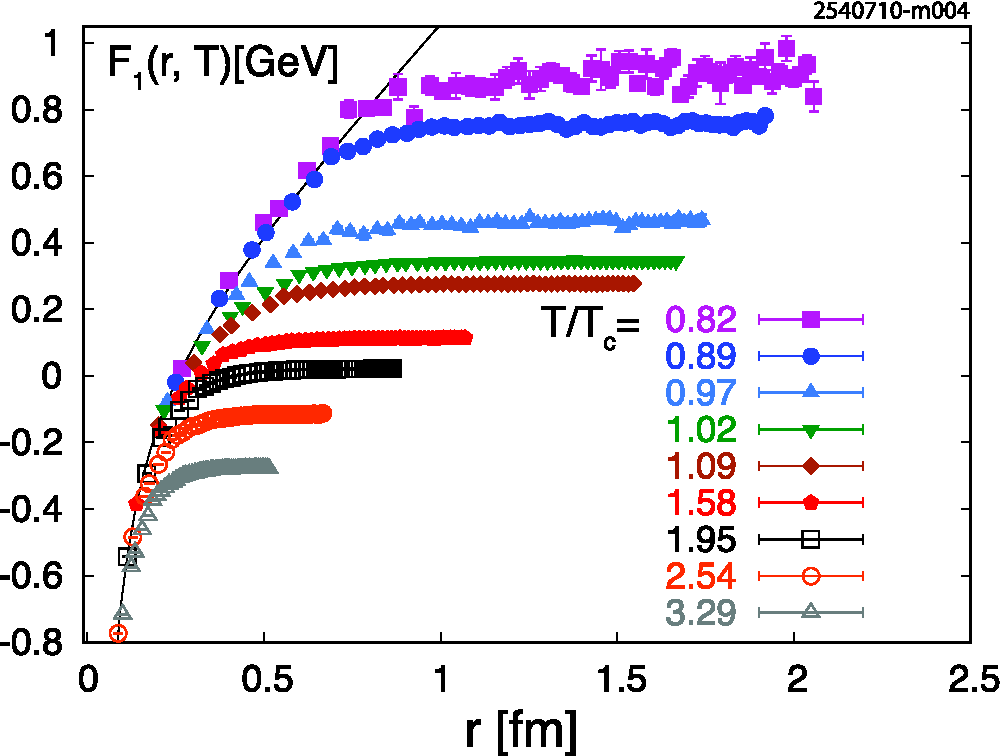
\includegraphics[width=0.6\textwidth]{Figures/LattSingEnergy.pdf}
      \caption{Heavy-quark-singlet free energy versus quark separation 
               calculated in 2+1 flavour QCD
              on $16^3 \times 4$ lattices at different 
               temperatures~\cite{Petreczky:2009ip,Petreczky:2010yn}  
               }
      \label{Fig:LatticeSingEner}
   \end{center}
\end{figure}
Color screening is studied on the lattice by 
calculating the spatial correlation function of a static quark and
antiquark in a color-singlet state which propagates in Euclidean time 
from $\tau=0$ to $\tau=1/T$, where $T$ is the temperature.
Lattice calculations of this quantity with dynamical quarks have been
reported~\cite{Kaczmarek:2002mc,Petreczky:2009ip,Petreczky:2010yn}.
The logarithm of the singlet
correlation function, also called the singlet free energy,
is shown in Fig.~\ref{Fig:LatticeSingEner}. 
As expected, in the zero-temperature limit the
singlet free energy coincides with the zero-temperature potential. 
Figure~\ref{Fig:LatticeSingEner} also illustrates that,
at sufficiently short distances, the singlet free energy is
temperature independent and equal to the zero-temperature potential. 
The range of interaction decreases with increasing temperature.  For 
temperatures above the transition temperature, $T_c$, the heavy-quark 
interaction range becomes comparable to the charmonium radius. Based on 
this general observation, one would expect that the charmonium
states, as well as the excited bottomonium states, do not remain bound at
temperatures just above the deconfinement transition, often referred to as 
{\em dissociation} or {\em melting}. 

%\subsubsection{Quarkonium spectral functions and quarkonium potential}
%\label{sec:media_subsec33}
In-medium quarkonium properties are encoded in the corresponding 
spectral functions, as is quarkonium dissociation
at high temperatures. Spectral functions are defined as
the imaginary part of the retarded correlation function of quarkonium
operators. Bound states appear as peaks in the spectral functions.
The peaks broaden and eventually disappear with
increasing temperature. The disappearance of a peak signals the melting of 
the given quarkonium state.
The quarkonium spectral functions can be calculated in potential models 
using the singlet free energy from Fig.~\ref{Fig:LatticeSingEner} or with different 
lattice-based potentials obtained using the singlet free energy
as an input~\cite{Mocsy:2007yj,Mocsy:2007jz}. 
The results for quenched QCD calculations are shown in Fig.~\ref{Fig:QuarkoniaSpecFuncLattice}
for S-wave charmonium (a) and bottomonium (b) 
spectral functions~\cite{Mocsy:2007yj}.
All charmonium states are dissolved in the deconfined phase while the bottomonium 1S
state may persist up to $T \sim 2T_c$. An upper bound on the dissociation temperature 
(the temperatures above which no
bound states peaks can be seen in the spectral function and bound state 
formation is suppressed) can be obtained from the analysis of the spectral 
functions. Conservative upper limits on the dissociation
temperatures for the different quarkonium states obtained from 
a full QCD calculation~\cite{Mocsy:2007jz} are given in Table~\ref{tab:LatticeDissTemp}.

\begin{figure}[]
   \begin{center}
      {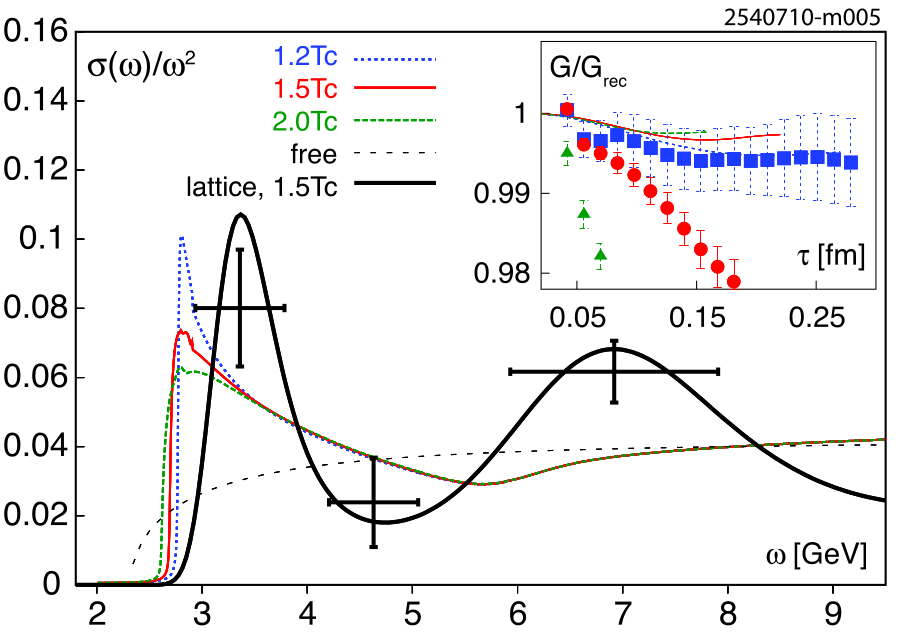
\includegraphics[width=0.49\textwidth]{Figures/JPsi_SpecFuncLattQCD.png}}
      {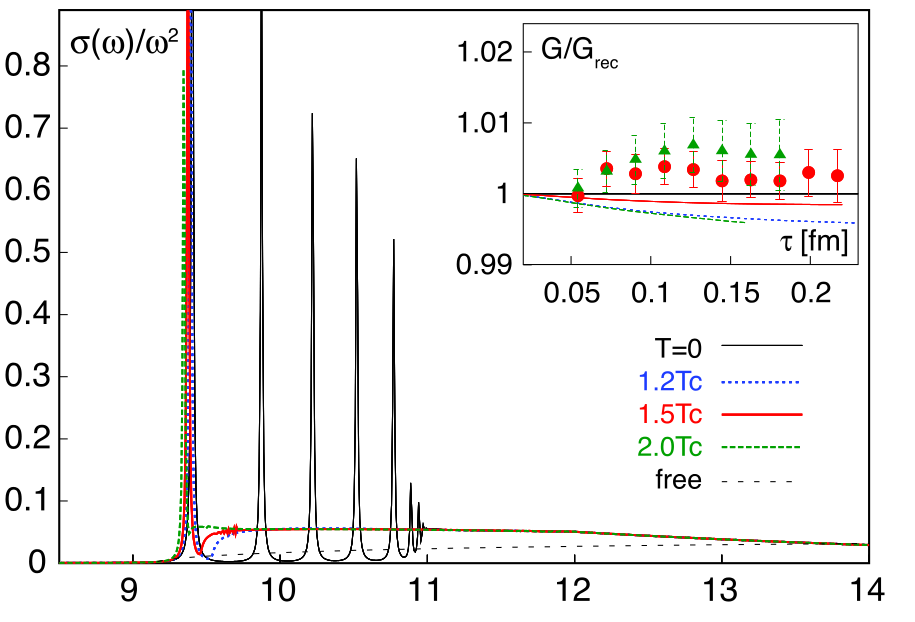
\includegraphics[width=0.49\textwidth]{Figures/Y1S_SpecFuncLattQCD.png}}
      \caption{The S-wave charmonium (a) and 
        bottomonium (b) spectral 
        functions calculated in potential 
        models. 
        Insets: correlators compared to lattice data.  
        The {\it dotted curves} are the
        free spectral functions.Figure is taken from Ref.~\cite{Mocsy:2007yj}.
      }
      \label{Fig:QuarkoniaSpecFuncLattice} 
   \end{center}
\end{figure}





\begin{table}[tb]
   \caption{Upper bounds on the dissociation 
             temperatures~\cite{Mocsy:2007jz}.
             }
   \label{tab:LatticeDissTemp}
   \setlength{\tabcolsep}{0.41pc}
   \begin{center}
      \begin{tabular}{ccccccc}
      \hline\hline
      %\rule[10pt]{-1mm}{0mm}
      State & $\chi_{cJ}(1P)$ & $\psi^{'}$ &J/$\psi$  &$\Upsilon(2S)$ & $\chi_{bJ}(1P)$ &$\Upsilon(1S)$ \\%[1.0mm]
      \hline 
      %\rule[10pt]{-1mm}{0mm}
      $T_{\rm diss}$ & $\le T_c$ & $\le T_c$ & $1.2T_c$ & $1.2T_c$ & $1.3T_c$ & $2T_c$\\ 
\hline\hline
\end{tabular}
\end{center}
\end{table}



%\subsubsection{Summary of hot medium effects}
%\label{sec:SummMedEff}
Potential model calculations based on lattice QCD, as well as resummed 
perturbative QCD calculations, indicate that all charmonium states and the
excited bottomonium states dissolve in the deconfined medium. This leads to 
the reduction of the quarkonium yields in heavy-ion collisions 
compared to the binary scaling of pp collisions. Recombination and edge
effects, however, guarantee a nonzero yield.


              
\subsection{Cold nuclear matter effects}
%{\color{red} This subsection will include the details of the models which use nuclear PDFs for quarkonia production
%like EPS19 or Color Glass Condensate modes. etc.~\cite{}. These effects are small for the Upsilon sector. }

The baseline for quarkonium production and suppression in heavy-ion collisions 
should be determined from studies of
cold-nuclear-matter (CNM) effects. The name cold matter 
arises because these effects are observed in hadron-nucleus interactions 
dense matter effects are much more important compared to the hot matter.  There are several 
CNM effects. The first such effect is the modifications of the parton 
distribution functions (PDF) in the nucleus compared to that in the nucleon. It depends mainly on two parameters, 
the momentum fraction of the parton $(x)$ and the scale of the parton-parton 
interaction $(Q^2)$. The nuclear density modified parton distributed function is known 
as nPDF. The nPDF to PDF ratio throws light on the modification quarkonia production 
in the CNM due to the modification of PDFs. This quantity is denoted as $R_i(x,Q^2)=f_i^{p \epsilon A} (x, Q^2) /
f_i^p  (x, Q^2)$. In the small x regime $(x < 10^{-2})$ this ration is less than unity. This feature is referred to as 
small-x shadowing. At intermediate x $(\sim 0.1)$ the ratio shows a hump like structure a phenomenon known as 
anti-shadowing. Around $x\approx 0.6$ one observes a dip which is known as EMC effect. The dynamics of partons 
within the nuclei is affected by the parton saturation which is successfully studied by color glass condensate. In the 
final state the quarkonia bound state scatter and re-scatter inelastically while passing through the nucleus. This leads 
the breakup or absorption of the bound state which is estimated by the inelastic cross-section of the quarkonia with 
the nucleon. 

Even though the contributions to CNM effects may 
seem rather straightforward, there are a number of associated uncertainties. 
First, while nuclear modifications of the quark densities are relatively 
well-measured in nuclear deep-inelastic scattering (nDIS), the modifications of the 
gluon density are not directly measured. The nDIS measurements probe only the 
quark and antiquark distributions directly. The scaling violations in nDIS can 
be used to constrain the nuclear gluon density. Overall momentum conservation 
provides another constraint. However, more direct probes of the gluon 
density are needed. Current shadowing parametrizations are derived from 
global fits to the nuclear parton densities and
give wide variations in the nuclear gluon 
density, from almost no effect to very large shadowing at low-$x$, 
compensated 
by strong antishadowing around $x \sim 0.1$.  

%The range of the possible shadowing effects is illustrated  in Fig. \ref{Fig:EPS09Shadowing} 
%by the new EPS09~\cite{Eskola:2009uj} parametrization and  its associated uncertainties, employing the scale values
% used to fix the \jpsi and \ups cross sections below the open-heavy-flavor threshold \cite{Frawley:2008kk}. 

%\begin{figure}
 % \begin{center}
 %   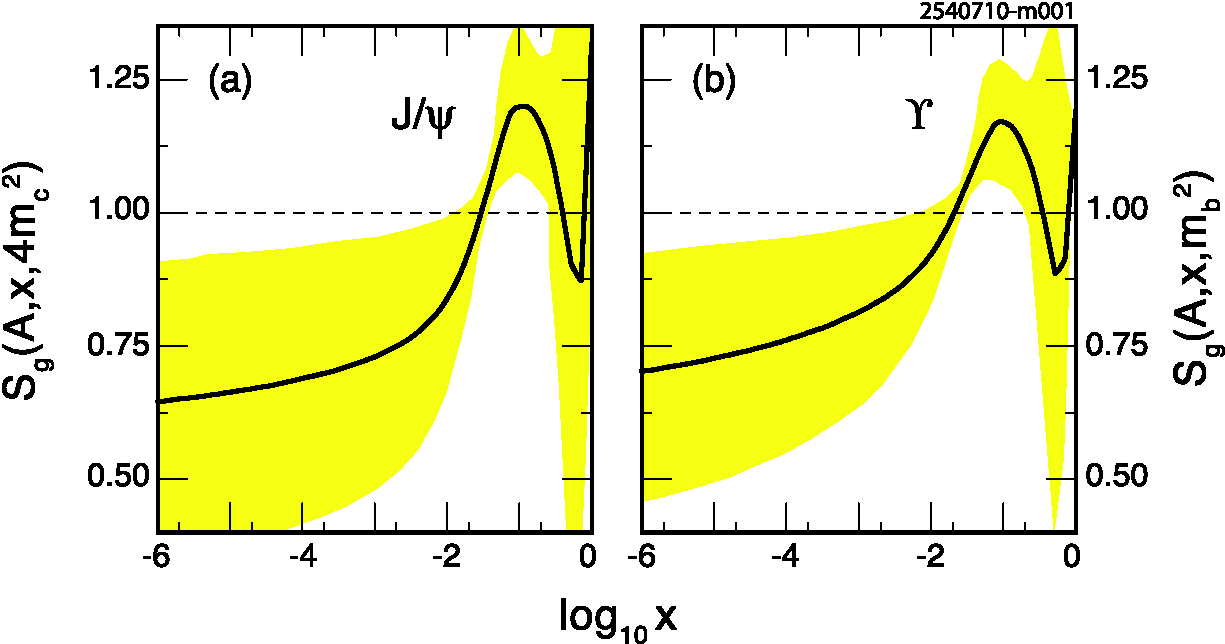
\includegraphics[width=0.9\textwidth]{Figures/EPS09GluonShadowing.pdf}
  %  \caption{The EPS09 gluon-shadowing parametrization~\cite{Eskola:2009uj} at $Q = 2m_{\rm c}$ 
%      and $m_{\rm b}$. The central value (solid curves) and the associated uncertainty
%      (shaded band) are shown }
 %   \label{Fig:EPS09Shadowing}
%  \end{center}
%\end{figure}


The nuclear absorption survival probability depends on the quarkonium 
absorption cross section. There are more inherent uncertainties 
in absorption than in the shadowing parametrization. It is obtained 
from data on other processes and is independent of the final 
state. Typically an absorption cross section is fit to the $A$ dependence 
of \jpsi and/or $\psi^{'}$ production in pA collision at a given energy. 
This is rather simplistic since it is unknown whether the object traversing the nucleus is a precursor 
color-octet state or a fully-formed color-singlet quarkonium state. The \jpsi absorption cross 
section at $y \sim 0$ is seen to decrease with energy, regardless of the chosen shadowing 
parametrization~\cite{Lourenco:2008sk}. 
% as shown in Fig.~\ref{Fig:AbsCrossVsE}.

%\begin{figure}[tb]
%   \begin{center}
%      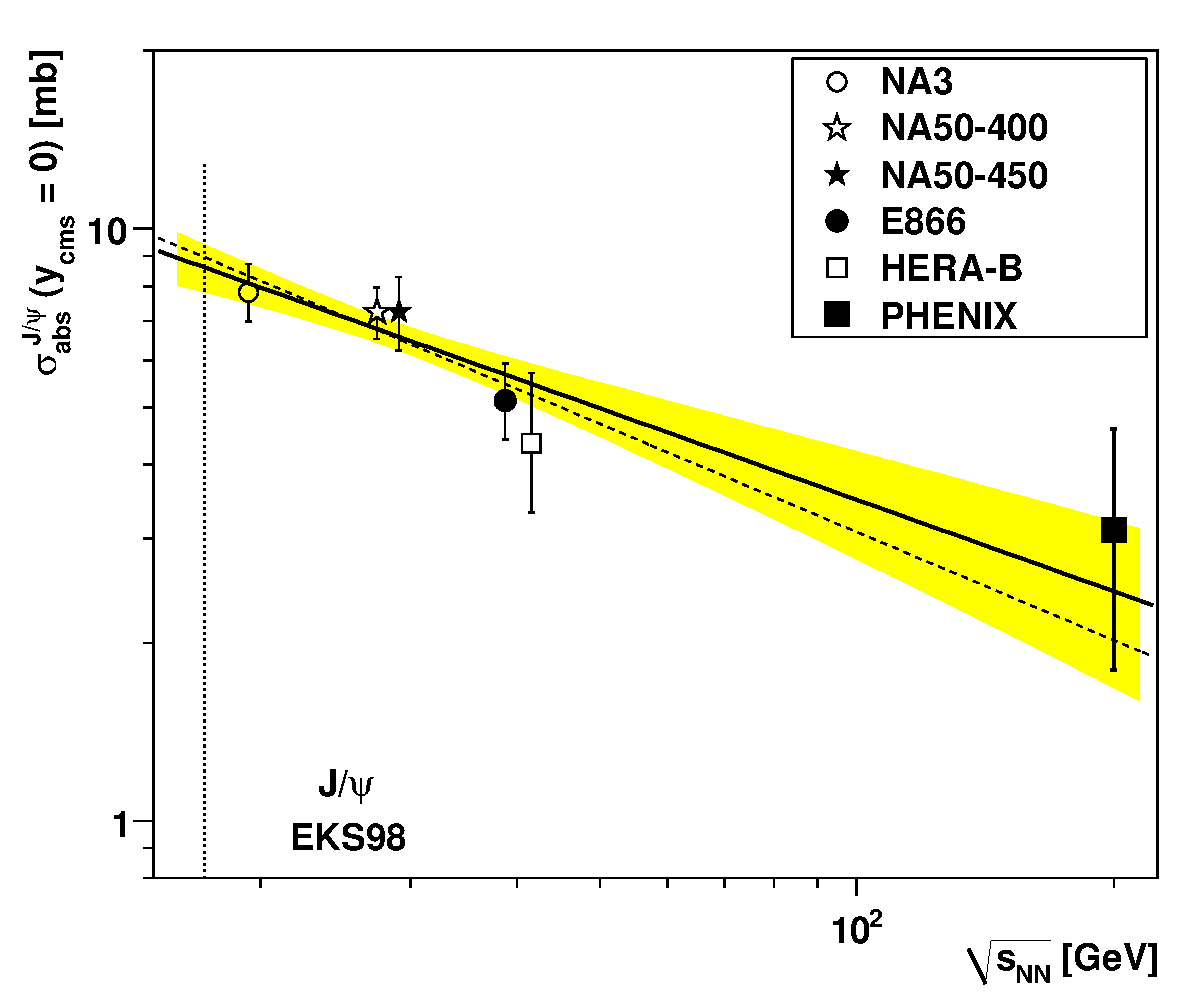
\includegraphics[width=0.6\textwidth]{Figures/AbsCrossVsE.pdf}
%      \caption{The extracted energy dependence of $\sigma_{\rm abs}^{\jpsi}$ at
 %              midrapidity.  The {\it solid line} is a 
 %              power law approximation 
 %              to $\sigma_{\rm abs}^{\jpsi}(y=0,\sqrt{s_{\rm NN}})$ using the 
 %              EKS98~{\protect\cite{Eskola:1998iy,Eskola:1998df}}
%               shadowing parametrization with the CTEQ61L parton densities
%               {\protect\cite{Pumplin:2002vw,Stump:2003yu}}.  
%               The {\it band} 
%               indicates the uncertainty in the extracted cross
%               sections.  The {\it dashed curve} shows an 
 %              exponential fit for comparison.  The data at
%               $y_{\rm cms} \sim 0$ from NA3~\cite{Badier:1983dg}, 
%               NA50 at 400\,GeV\,{\protect\cite{Alessandro:2006jt}} and 
%               450\,GeV\,\cite{Alessandro:2003pc},
%               E866~\cite{Leitch:1999ea}, 
 %              HERA-B~\cite{Abt:2008ya}, and
%               PHENIX~\cite{daSilva:2009yy} are also shown.  
%               The {\it vertical dotted line} indicates the energy 
%               of the Pb+Pb and In+In collisions at the
%               CERN SPS. Figure is take from Ref.~\cite{Lourenco:2008sk} 
%      }
 %     \label{Fig:AbsCrossVsE}
%   \end{center}
%\end{figure}



Recent analyses of $\jpsi$ production
in fixed-target interactions~\cite{Lourenco:2008sk} 
show that the effective absorption
cross section depends on the energy of the initial beam and the rapidity or
$x_F$ of the observed $\jpsi$.  One possible interpretation is that 
low-momentum color-singlet states can hadronize in the
target, resulting in larger effective absorption cross sections at lower
center-of-mass energies and backward $x_F$ (or center-of-mass rapidity).
At higher energies, the states traverse the target more rapidly so that
the $x_F$ values at which they can hadronize in the target move 
back from midrapidity toward more negative $x_F$.
Finally, at sufficiently high energies, the quarkonium states pass 
through the target before hadronizing, resulting in negligible absorption
effects.  Thus the {\it effective} absorption cross section decreases with 
increasing center-of-mass energy because faster states are less likely 
to hadronize inside the target.
%It is also well known that feeddown 
%from $P$ and higher-$S$ states through radiative 
%and hadronic transitions, respectively,
%accounts for almost half of the observed J/$\psi$ and $\Upsilon(1S)$ 
%yields. The excited quarkonium states have very 
%different sizes and formation times 
%and should thus have different absorption cross sections.

This is a very simplistic picture. In practice, cold-nuclear-matter effects 
(initial-state energy loss, shadowing, final-state breakup, {\it etc.}) 
depend differently on the quarkonium kinematic variables and the collision energy. 
It is clearly unsatisfactory to combine all these mechanisms into an {\it effective} 
absorption cross section, as employed in the Glauber formalism, 
that only evaluates final-state absorption. 
Simply taking the $\sigma_{\rm abs}$ obtained from 
the analysis of the pA data 
and using it to define the Pb+Pb baseline is not be sufficient. 
A better understanding of absorption requires more detailed knowledge of the 
production mechanisms which it self are largely unknown.






\subsection{Kinetic approach}

{\color{black}

  In the kinetic approach \cite{Thews:2000rj}, the proper time $\tau$ evolution of the quarkonia 
  population $N_{Q}$
  is given by the rate equation 
  
  \begin{equation}\label{eqkin}
    {dN_{Q} \over d\tau}  =  - \lambda_D  \rho_g N_{Q} + \lambda_F {N_{q \bar{q}}^{2} \over V(\tau)},
  \end{equation}
  where $V(\tau)$ is the volume of the deconfined spatial region and $N_{q \bar{q}}$ is the number of initial 
  heavy quark pairs produced per event depending on the centrality defined by the number of participants
  $N_{\rm part}$.
  The $\lambda_{D}$ is the dissociation rate obtained by the dissociation cross section averaged over 
  the momentum 
  distribution of gluons and $\lambda_{F}$ is the formation rate obtained by the formation cross section 
  averaged over the momentum distribution of heavy quark pair $q$ and $\bar{q}$. 
  $\rho_g$ is the density of thermal gluons.
  The number of quarkonia at freeze-out time $\tau_f$ is given by the solution of Eq.~(\ref{eqkin}),
  \begin{equation}
    N_{Q}(p_T) = S(p_T) \,N_{Q}^{\rm PbPb}(p_T)+N_{Q}^F(p_T).
    \label{eqbeta}
  \end{equation}
  Here $N_{Q}^{\rm PbPb}(p_T)$ is the number of initially-produced quarkonia (including shadowing)
  as a function of $p_T$ and $S(p_T)$ is their survival probability from gluon collisions at freeze-out, 
  \begin{equation}
    S(p_T) = \exp \left( {-\int_{\tau_0}^{\tau_f}f(\tau) \lambda_{\rm D}(T,p_T)\,\rho_g(T)\,d\tau} \right).
  \end{equation}
  The temperature $T(\tau)$ and the QGP fraction $f(\tau)$ evolve from initial time $\tau_0$ 
  to freeze-out time $\tau_f$ due to expansion of the QGP. The initial temperature and the 
  evolution is dependent on collision centrality $N_{\rm part}$.
  $N_{Q}^F(p_T)$ is the number of regenerated quarkonia per event,
  \begin{equation}
    N_{Q}^F(p_T)=S(p_T)N_{q \bar{q}}^{2} \int_{\tau_0}^{\tau_f}{{\lambda_{\mathrm{F}}(T,p_T) \over V(\tau)\,S(\tau,p_T)} d\tau}.
  \end{equation}
  The nuclear modification factor ($R_{AA}$) can be written as 
  \begin{equation}
    R_{AA}(p_T)=S(p_T) \, R(p_T) + \frac{N_{Q}^F(p_T)}{N_{Q}^{pp}(p_T)}.
    \label{raa}
  \end{equation}
  Here $R(p_T)$ is the shadowing factor.
%  $R_{AA}$ as a function of collision centrality, including regeneration, is
%  \begin{equation}
%    R_{AA}(N_{\rm part}) = \frac{\int_{p_{T\,\rm cut}} N_{Q}^{pp}(p_T)S(p_T)\, R(p_T) dp_T}{\int_{p_{T\,\rm cut}} N_{Q}^{pp}(p_T) dp_T} + 
%    \frac{\int_{p_{T\, \rm cut}} N_{Q}^F(p_T) dp_T}{\int_{p_{T\, \rm cut}} N_{Q}^{pp}(p_T) dp_T}
%    \label{raa2}
%  \end{equation}
%  Here $p_{T~{\rm cut}}$ defines the $p_T$ range for a given experimental acceptance.
%  $N_{Q}^{pp}(p_T)$ is the unmodified $p_T$ distribution of quarkonia obtained by NLO 
%  calculations and scaled to a particular centrality of the Pb+Pb collisions.
  


  In the color dipole approximation, the gluon dissociation cross section as function of gluon energy, $q^0$,
  in the quarkonium rest frame is~\cite{Bhanot:1979vb}
  \begin{equation}
    \sigma_{D}(q^{0}) = {8\pi \over 3} \, {16^2 \over 3^2} {a_0 \over m_q}  \frac{(q^0/\epsilon_0 - 1)^{3/2}} {(q^0/\epsilon_0)^5},
  \end{equation}
  where $\epsilon_0$ is the quarkonia binding energy and $m_q$ is the charm/bottom quark mass 
  and $a_0=1/\sqrt{m_q\epsilon_0}$.
  The values of $\epsilon_0$ are taken as 0.64 and 1.10 GeV for the ground states, $\Jpsi$ and $\Upsilon$(1S),
  respectively \cite{Karsch:1987pv}.
  For the first excited state of bottomonia, $\Upsilon$(2S), we use dissociation
  cross section from Ref.~\cite{Arleo:2001mp}.

  \begin{figure}
    \begin{center}
    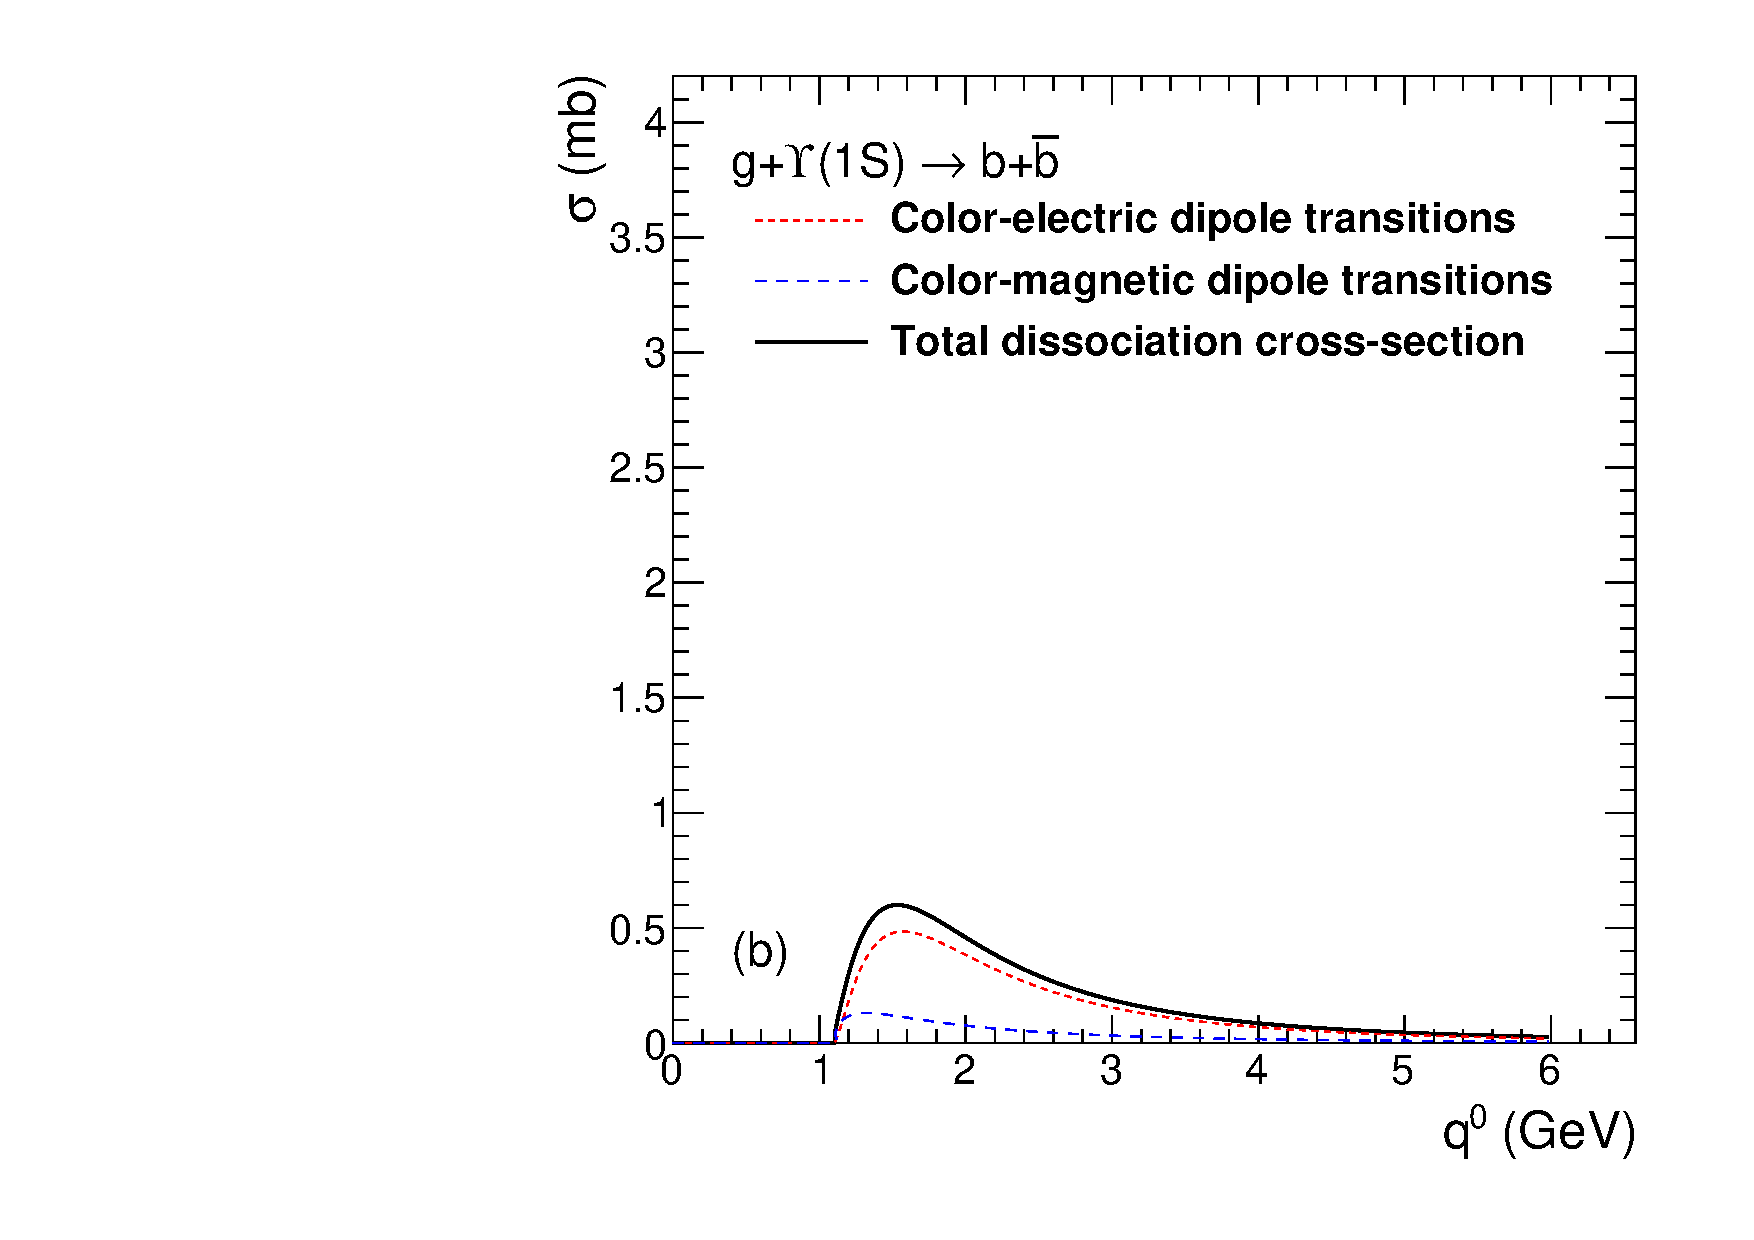
\includegraphics[width=0.50\textwidth]{Figures/Quarkonia_502TeV/Fig1b_Y1S_SigmaDq0.pdf}
    \caption{(Color online) Gluon dissociation cross section of quarkonia as a function of gluon energy ($q^{0}$) in
      quarkonia rest frame.}
    \label{fig:SigmaDQ0}
    \end{center}
  \end{figure}

  
  Figure \ref{fig:SigmaDQ0} shows the gluon dissociation cross sections of $\Jpsi$ and $\Upsilon$(1S)
  as a function of gluon energy. The dissociation cross section is zero when the gluon energy is less 
  than the binding energy of the quarkonia. It increases with gluon energy and reaches a maximum at 1.2 (1.5) GeV for 
  $\Jpsi~(\Upsilon(1{\rm S}))$. At higher gluon energies, the interaction probability decreases. The gluon energy $q^0$ 
  is related to the square of the center of mass energy $s$, of the quarkonium-gluon system by
  \begin{eqnarray}
    q^{0} = \frac{s-M_{Q}^{2}}{2\,M_{Q}}
  \end{eqnarray}  
  where $M_{Q}$ ais the mass of quarkonium.  We calculate the dissociation rate as a function of quarkonium momentum 
  by integrating the dissociation cross section over thermal gluon momentum 
  distribution $f_{g}(p_g)$.


  We can calculate the formation cross section from the dissociation cross section using
  detailed balance~\cite{Thews:2000rj,Thews:2005vj},
  \begin{equation}
    \sigma_{F} = \frac{48}{36}\,\sigma_{D}(q^0)\frac{(s-M_{Q}^2)^{2}}{s(s-4m_q^{2})}.
  \end{equation}
  The formation rate of quarkonium with momentum {\bf p} can be obtained using
  thermal distribution functions of  $q/\bar{q}$.
  
  

%%%%%%%%%%%%%%%%%%%%%%%%%%%%%%%%%%%%%%%%%%%%%%%%%%%%%%%% 5.02 TeV %%%%%%%%%%%%%%%%%%%%%%%%%%%%%%%%%%%%%%%%%
\begin{figure}
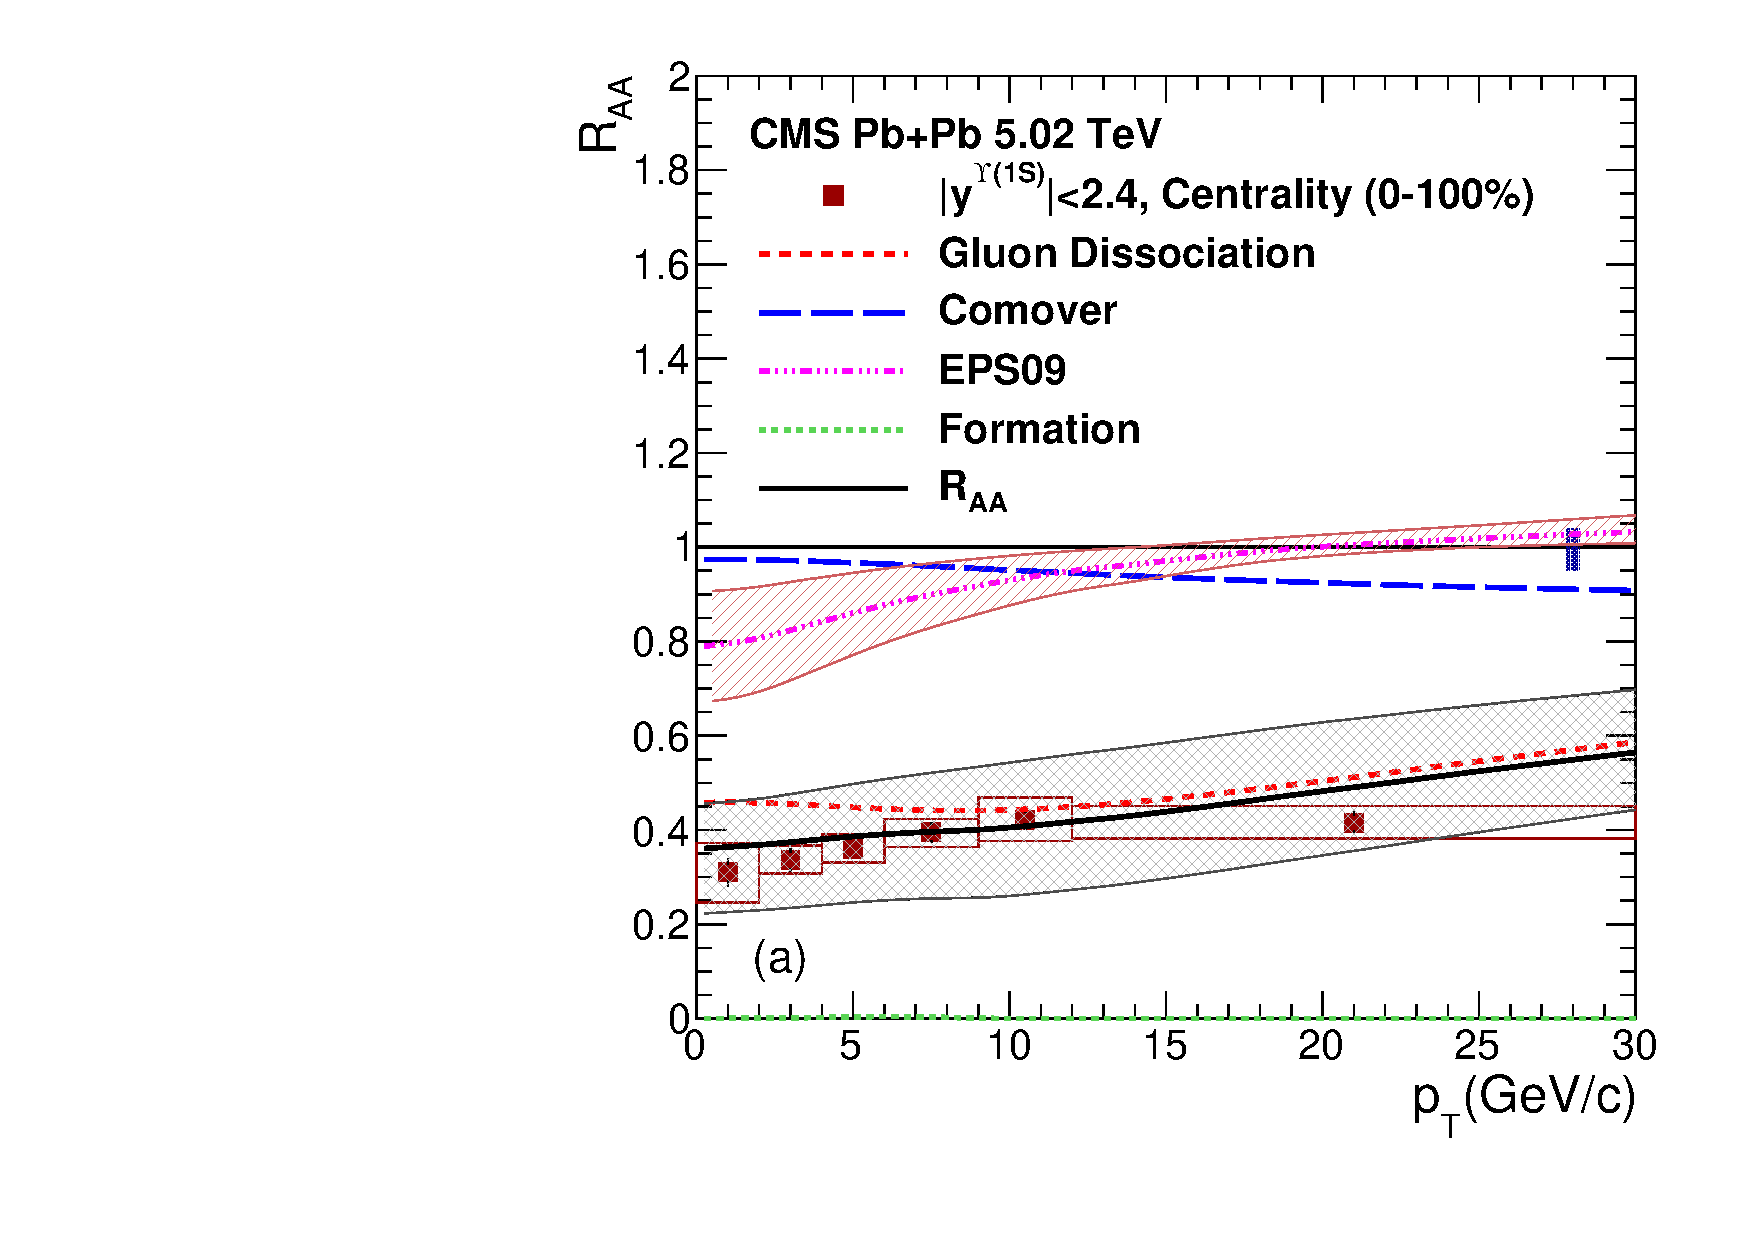
\includegraphics[width=0.49\textwidth]{Figures/Quarkonia_502TeV/Fig7a_Y1S_CMS_RAAPt_Shade.pdf}
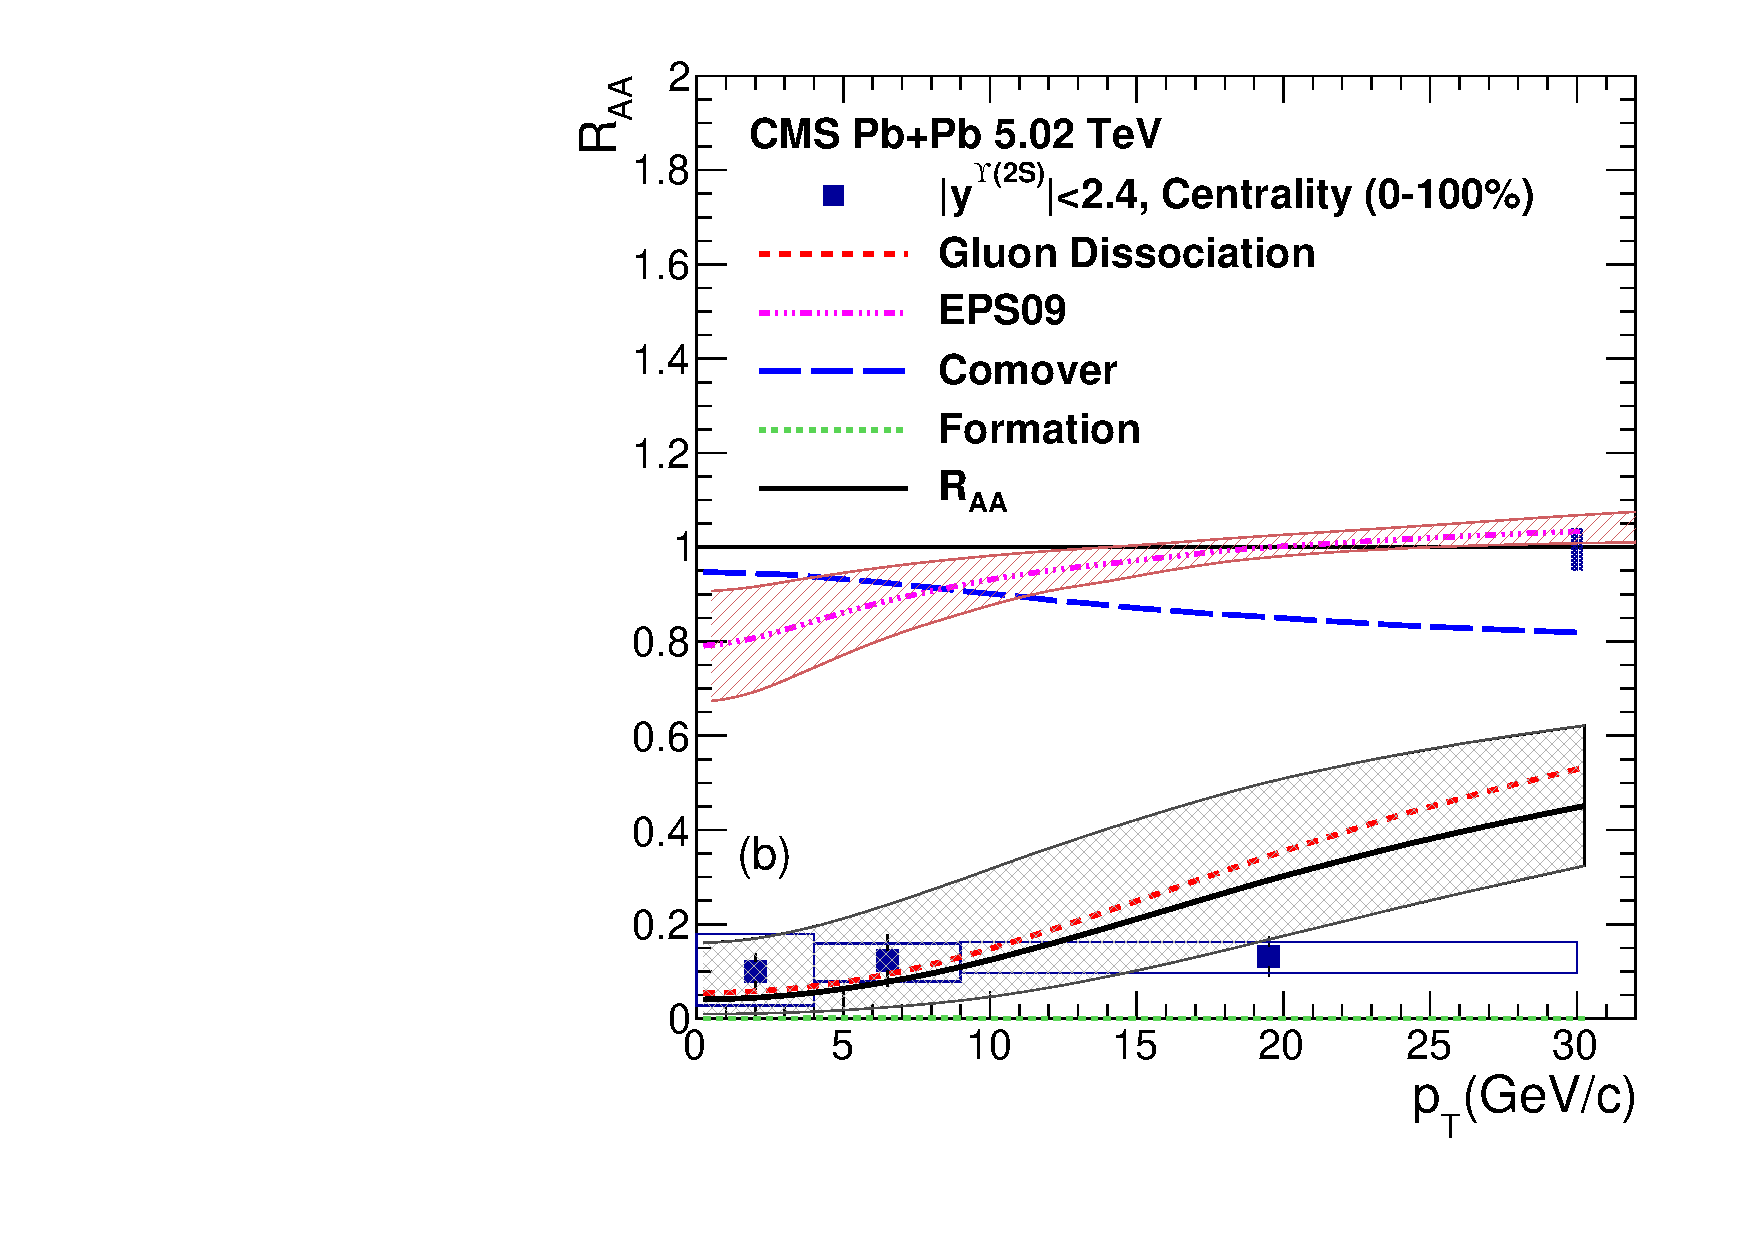
\includegraphics[width=0.49\textwidth]{Figures/Quarkonia_502TeV/Fig7b_Y2S_CMS_RAAPt_Shade.pdf}
\caption{(Color online) Calculated nuclear modification factor ($R_{AA}$) of (a) $\Upsilon$(1S) and 
  (b) $\Upsilon$(2S) as a function of $p_{T}$ 
  compared with CMS measurements~\cite{Sirunyan:2018nsz}.
The global uncertainty in $R_{AA}$ is shown as a band around the line at 1.
}
\label{fig:UpsilonRaaPtCMS}
\end{figure}



\begin{figure}
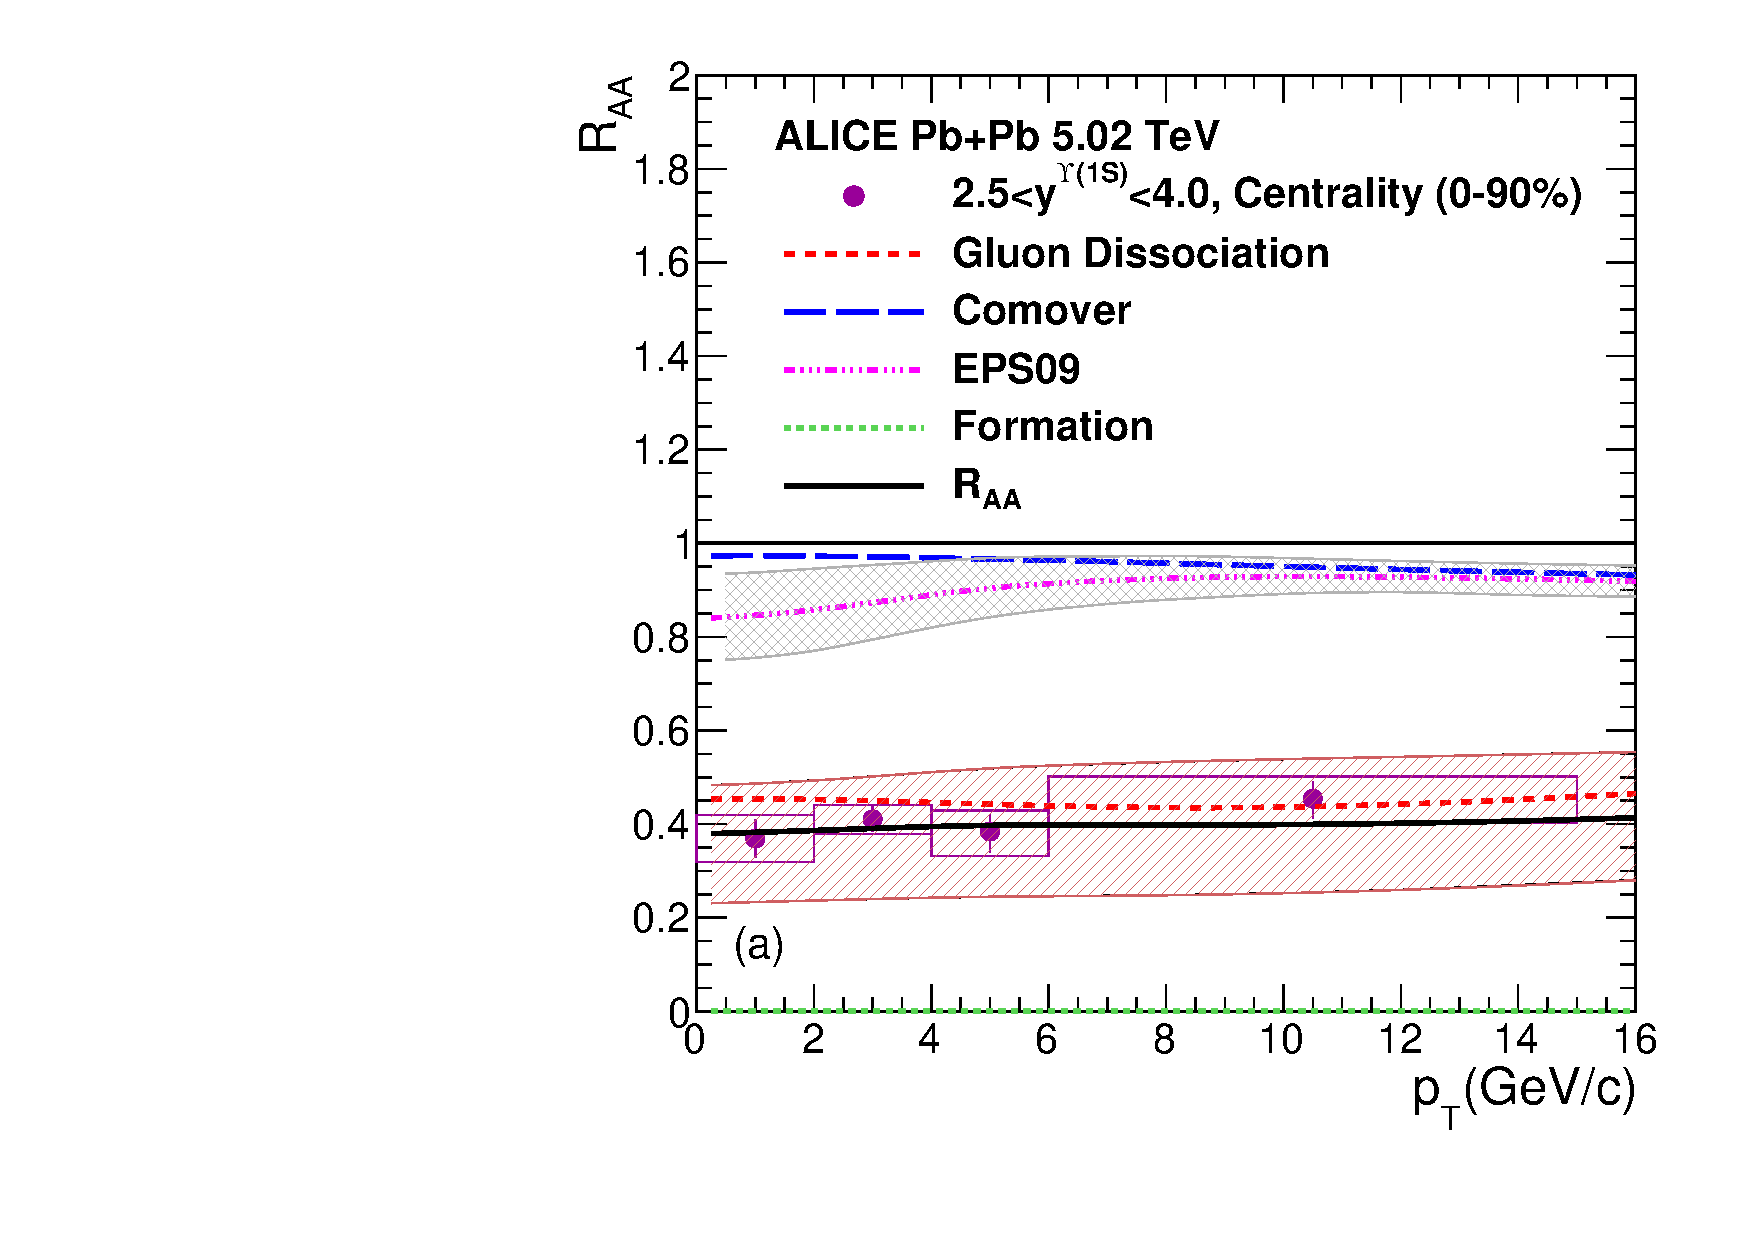
\includegraphics[width=0.49\textwidth]{Figures/Quarkonia_502TeV/Fig8a_ALICE_Y1SRAAPt_Shade.pdf}
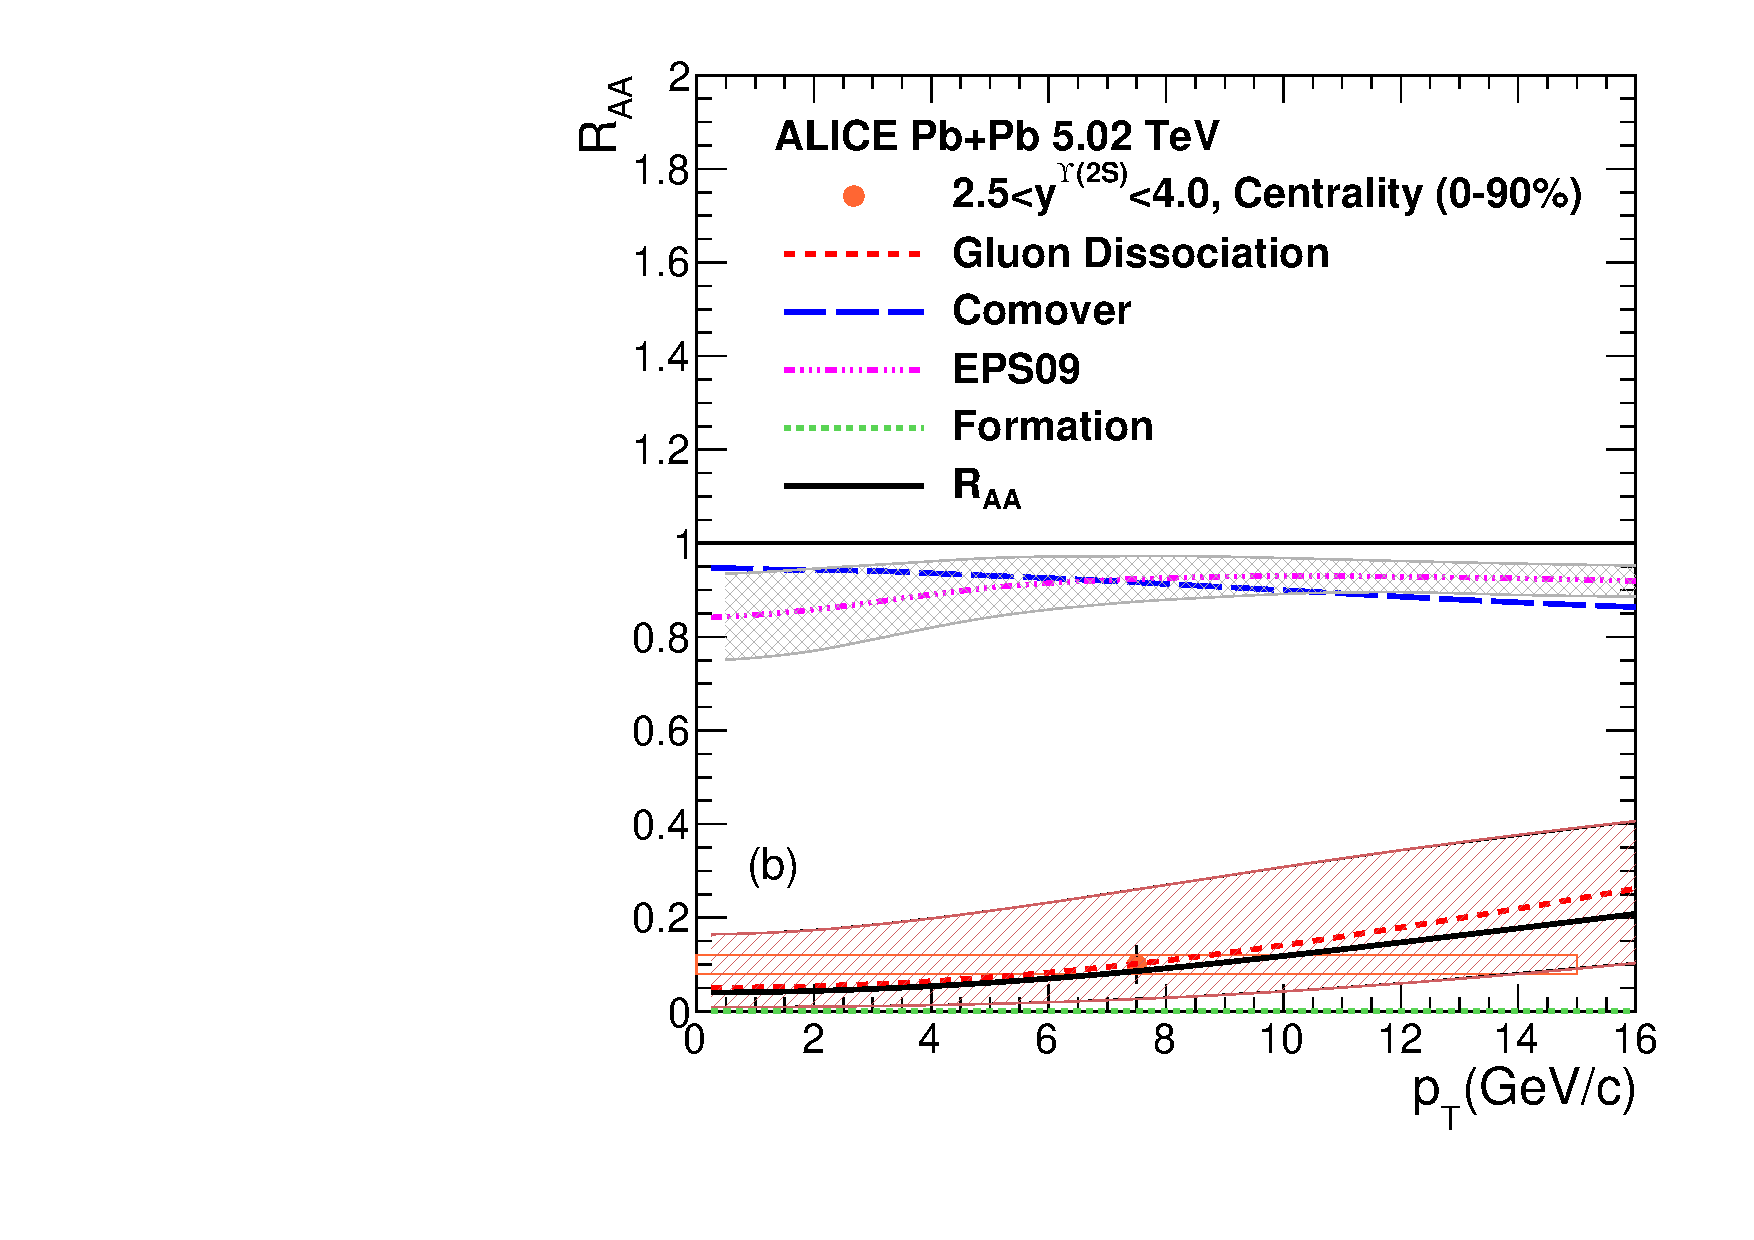
\includegraphics[width=0.49\textwidth]{Figures/Quarkonia_502TeV/Fig8b_ALICE_Y2SRAAPt_Shade.pdf}
\caption{(Color online) Calculated nuclear modification factor ($R_{AA}$) of (a) $\Upsilon$(1S) and 
  (b) $\Upsilon$(2S) as a function of $p_{T}$ in the kinematic range of ALICE detector at LHC ~\cite{ALICE:2020wwx}.
  The global uncertainty in $R_{AA}$ is shown as a band around the line at 1.
} 
\label{fig:UpsilonRaaPtALICE}
\end{figure}

\begin{figure}
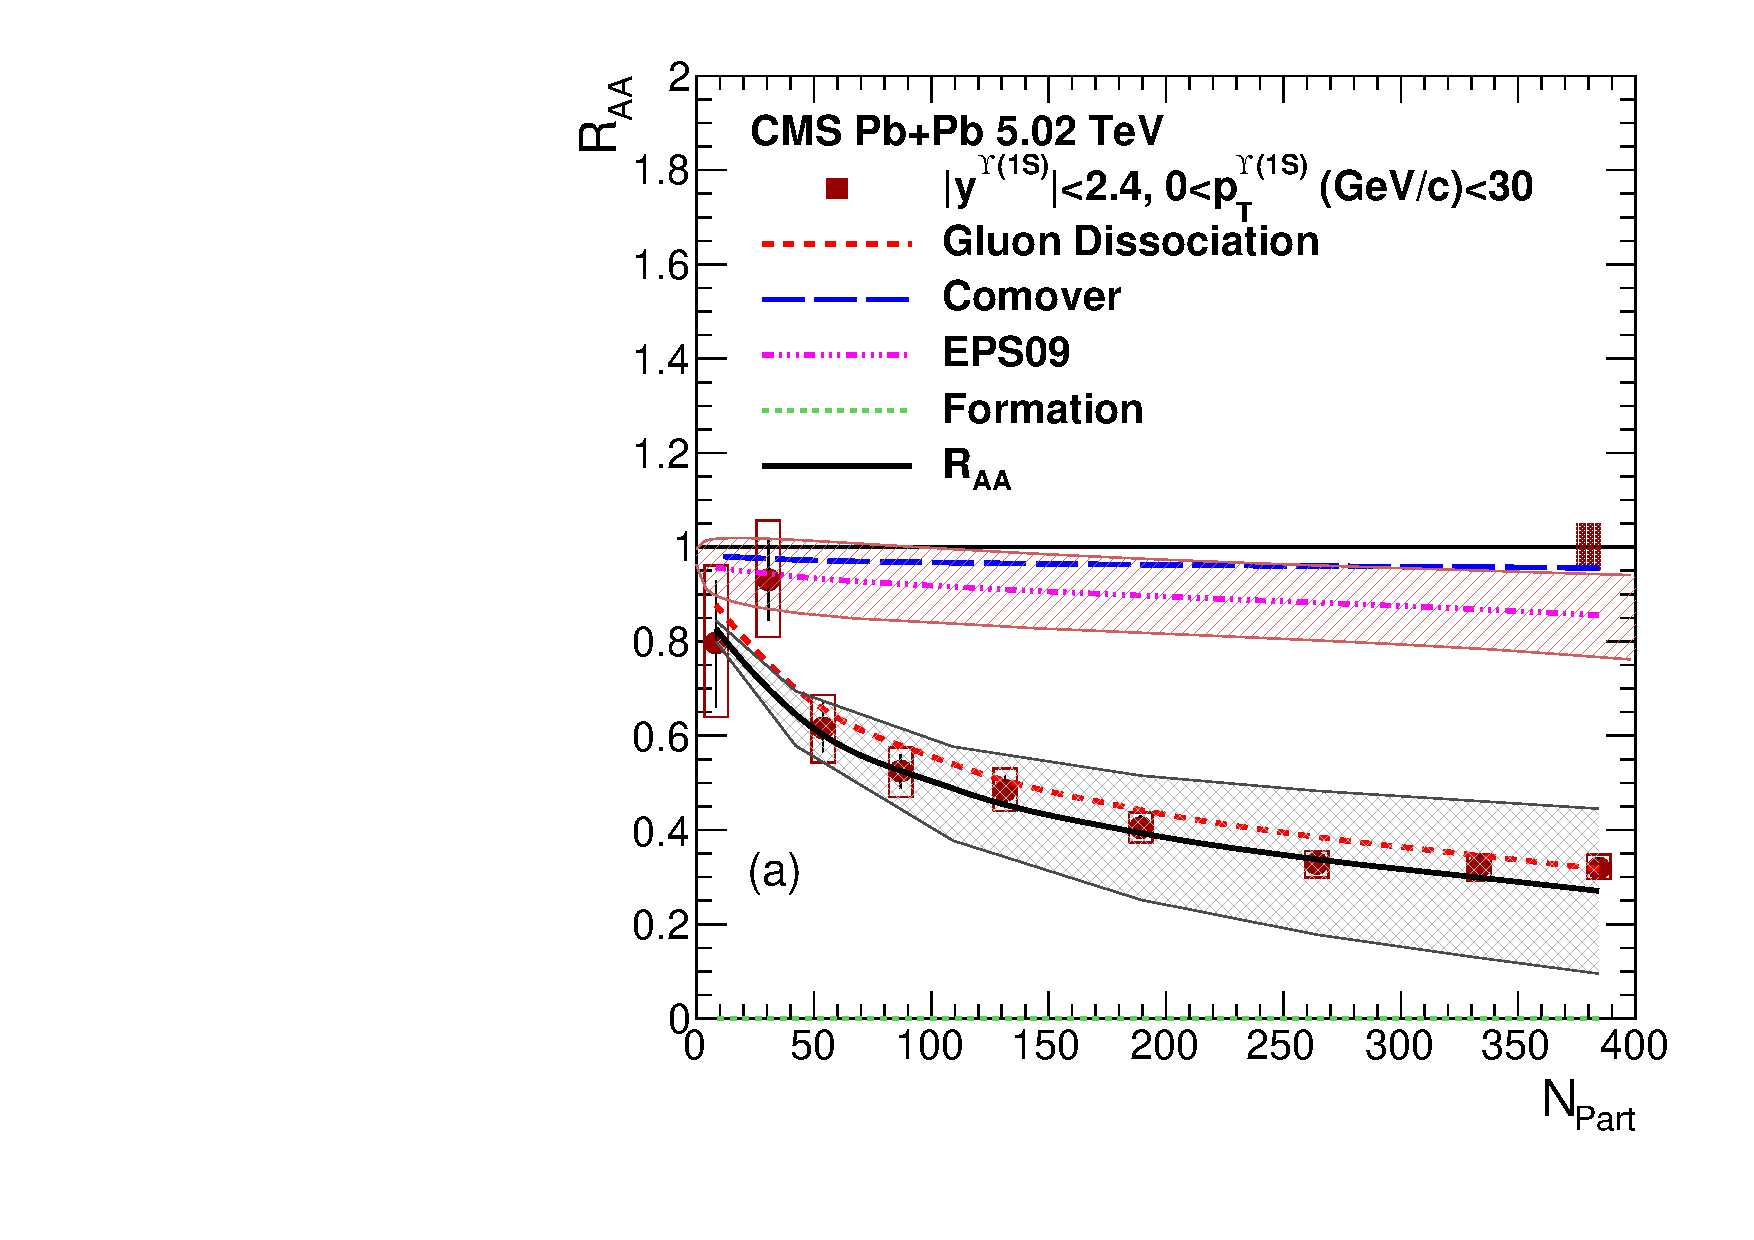
\includegraphics[width=0.49\textwidth]{Figures/Quarkonia_502TeV/Fig9a_CMS_Y1SRAANPart_Shade.pdf}
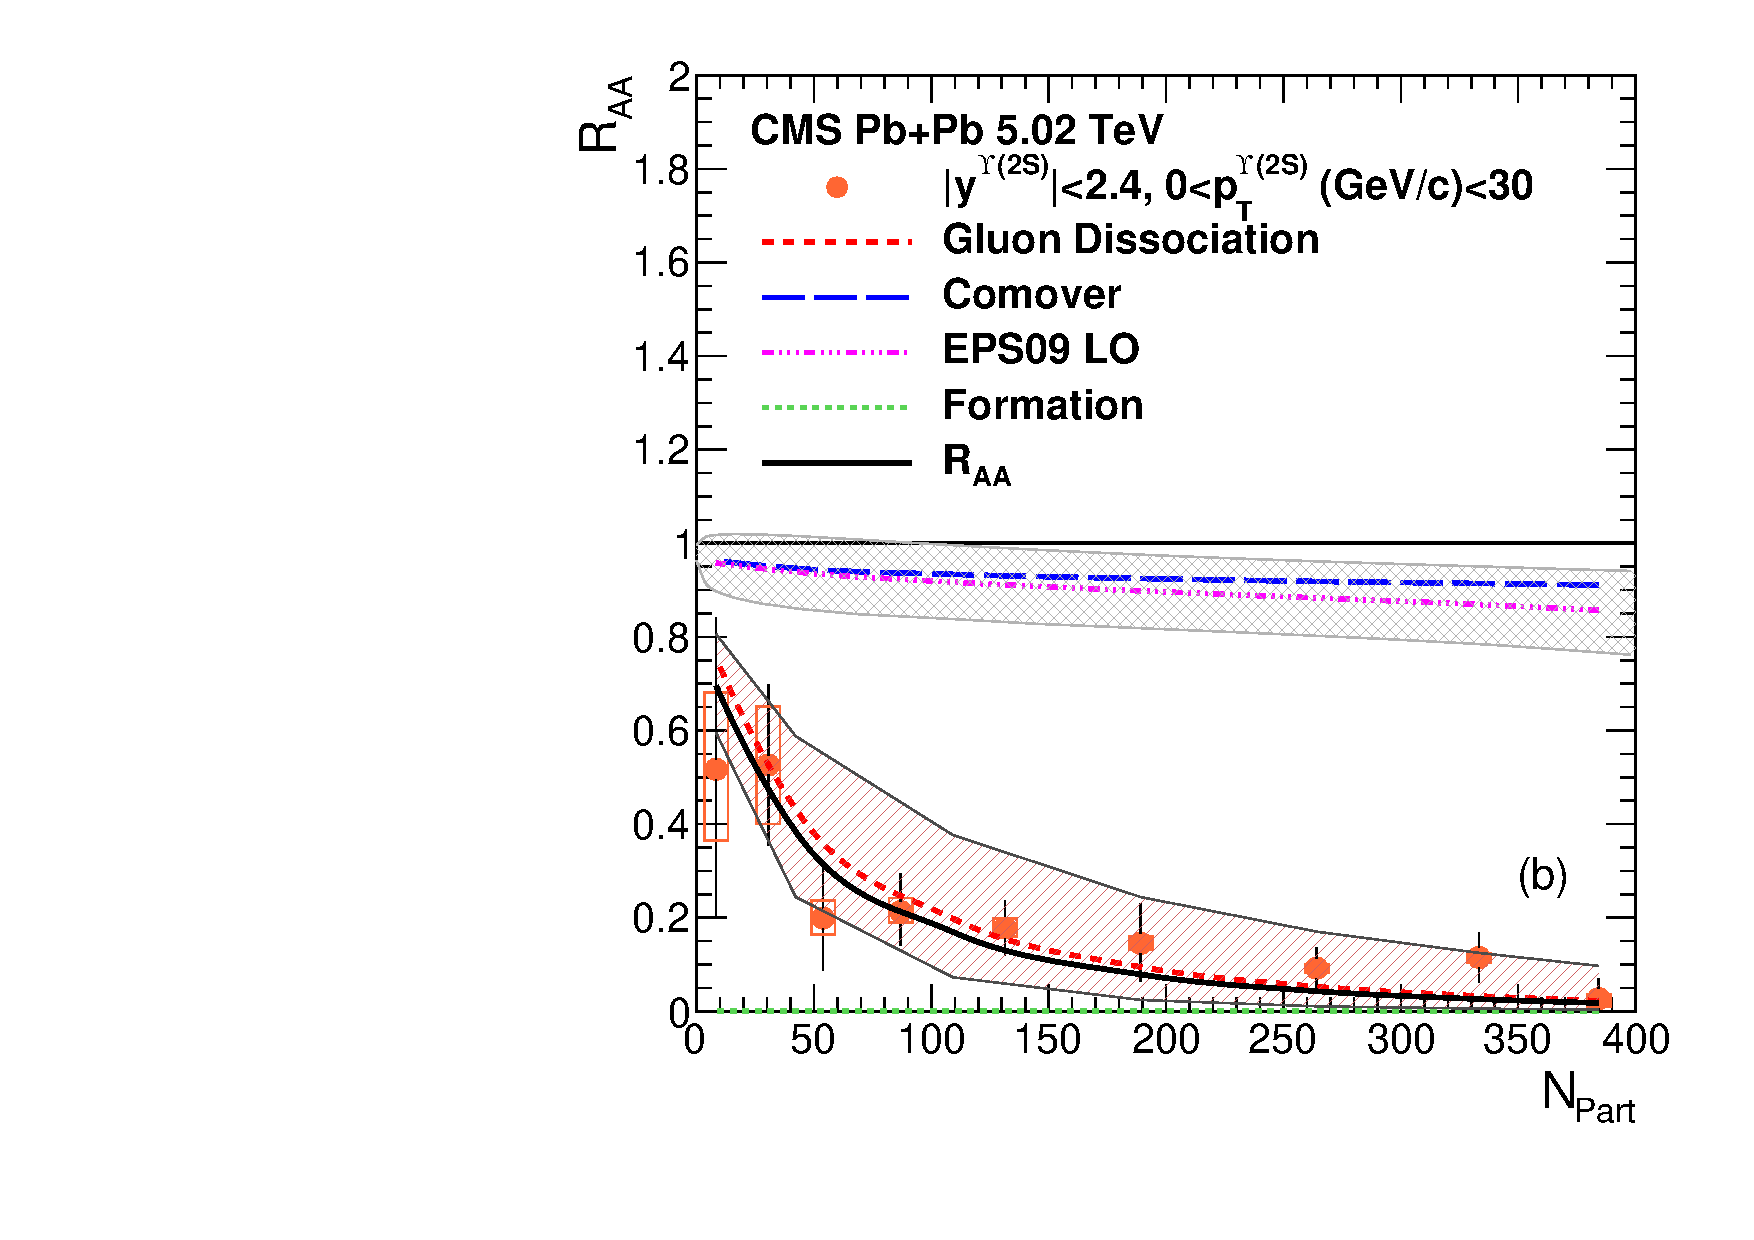
\includegraphics[width=0.49\textwidth]{Figures/Quarkonia_502TeV/Fig9b_CMS_Y2SRAANPart_Shade.pdf}
\caption{(Color online) Calculated nuclear modification factor ($R_{AA}$) of 
  (a) $\Upsilon$(1S) and (b) $\Upsilon$(2S) as a function of centrality of the 
  collisions compared with the CMS measurements~\cite{Sirunyan:2018nsz}.%\cite{CMS:2017ucd}.
  The global uncertainty in $R_{AA}$ is shown as a band around the line at 1.
}
\label{fig:UpsilonRaaNPartCMS}
\end{figure}


Figure~\ref{fig:UpsilonRaaPtCMS}(a) and (b) show the calculations of contributions to
the nuclear modification factor, $R_{AA}$, for the $\Upsilon$(1S) and $\Upsilon$(2S)
respectively as a function of $p_T$ compared with the mid rapidity measurements from
CMS~\cite{Sirunyan:2018nsz}.  
The gluon dissociation mechanism combined with the pion dissociation and shadowing
corrections gives good description of data in mid $p_{T}$ range ($p_{T}\approx$ 5-10 GeV/c)
for both $\Upsilon$(1S) and $\Upsilon$(2S).
The contribution from the regenerated $\Upsilon$s is negligible even at LHC energies.
Our calculations under-predict the suppression observed at the highest measured
$p_{T}$ for $\Upsilon$(1S) and $\Upsilon$(2S) which is similar for the case
of J/$\psi$.
%The feed-down corrections are applied in our calculations following the similar
%procedure as in Refs.~\cite{Abdulsalam:2012bw,Krouppa:2017jlg}. 
%%%%%%%%% insert the feed-down details here
The states $\Upsilon$(1S) and $\Upsilon$(2S) also have
feed-down contributions from decays of higher b$\bar{\rm b}$ bound states.
The nuclear modification factor, $R_{AA}$ is obtained taking into account the feed-down corrections as follows
  \begin{equation}
    R_{AA}^{\Upsilon(3S)} = R_{AA}^{\Upsilon(3S)}\\ %\nonumber
  \end{equation}
  \begin{equation}
    R_{AA}^{\Upsilon(2S)} = f_1 R_{AA}^{\Upsilon(2S)} +  f_2 R_{AA}^{\Upsilon(3S)} \\ %\nonumber
  \end{equation}
   \begin{equation}
    R_{AA}^{\Upsilon(1S)} = g_1 R_{AA}^{\Upsilon(1S)} +  g_2 R_{AA}^{\chi_b(1P)} + g_3 R_{AA}^{\Upsilon(2S)} + g_4 R_{AA}^{\Upsilon(3S)}\\ %\nonumber
  \end{equation}
The factors $f$'s and $g$'s are obtained from CDF measurement~\cite{Affolder:1999wm}.
The values of $g_1$, $g_2$, $g_3$ and $g_4$ are 0.509, 0.27, 0.107
and 0.113 respectively. Here $g_4$ is assumed to be the combined fraction of 
$\Upsilon$(3S) and $\chi_b$(2P).
The values of $f_1$ and $f_2$ are taken as 0.50~\cite{Strickland:2011aa}.


Figure~\ref{fig:UpsilonRaaPtALICE}(a) and (b) show the model 
prediction of the nuclear modification factor, $R_{AA}$, for the $\Upsilon$(1S)
and $\Upsilon$(2S) respectively as a function of $p_T$ in the kinematic range
covered by ALICE detector. The ALICE data~\cite{ALICE:2020wwx} is well described by our model.

Figure~\ref{fig:UpsilonRaaNPartCMS}(a) depicts the calculated 
centrality dependence of the $\Upsilon$(1S) nuclear
modification factor, along with the midrapidity data from CMS~\cite{Sirunyan:2018nsz}.
Our calculations combined with the pion dissociation and shadowing corrections 
gives very good description of the measured data. Figure~\ref{fig:UpsilonRaaNPartCMS}(b)
shows the same for the $\Upsilon$(2S) along with the midrapidity
CMS measurements. The suppression of the excited $\Upsilon$(2S) states 
is also well described by our model. As stated earlier, the effect of regeneration is
negligible for $\Upsilon$ states. 


  The suppression of quarkonia by comoving pions can be calculated by folding the quarkonium-pion
dissociation cross section $\sigma_{\pi Q}$ over thermal pion distributions \cite{Vogt:1988fj}. 
It is expected  that at LHC energies, the comover cross section will be small~\cite{Lourenco:2008sk}.
{\color{black}
The pion-quarkonia cross section is calculated by convoluting the gluon-quarkonia cross section $\sigma_D$
over the gluon distribution inside the pion~\cite{Arleo:2001mp},
\begin{equation}
\sigma_{\pi Q} (p_{\pi}) = {p_+^2 \over 2(p_\pi^2 - m_\pi^2)} \int_0^1 \, dx \, G(x) \, \sigma_D(xp_+/\sqrt {2}),
\end{equation}
where $p_+ = (p_\pi + \sqrt{p_\pi^2-m_\pi^2})/\sqrt{2}$. The gluon distribution, $G(x)$, inside a pion is 
given by the GRV parameterization~\cite{Gluck:1991ey}. 
The dissociation rate $\lambda_{D_{\pi}}$  can be obtained using the 
thermal pion distribution.


\subsection{Transport approach in bottomonia production }

There have been some studies in looking at the transport approach to the bottomonia 
production.~\cite{Grandchamp:2005yw,Rapp:2017chc}. This 
is an approach of studying the rate equations. Such an equation for bottomonium production  in the medium's rest frame can be written as~\cite{Grandchamp:2005yw},
\begin{equation}
\frac{\mathrm{d} N_Y(\tau)}{\mathrm{d}\tau} =
-\Gamma_Y(T)\left[N_Y(\tau)-N^{\rm eq}_Y(T)\right] \ ,
\end{equation}
In the above equation $\Gamma_Y$, is the inelastic reaction rate  and $N^{\rm eq}_Y(T)$ is the thermal equilibrium limit  for each state $Y=\Upsilon(1S), \Upsilon(2S), \chi_c, ...$.

In the reaction rates  both gluo-dissociation and quasi-free mechanisms have been incorporated.  An important 
ingredient in this calculation is the bottomonium binding energies. 
The thermal-equilibrium limit is evaluated from the statistical model with bottom ($b$) quarks~\cite{Grandchamp:2002wp}. 
The initial conditions are obtained from the $pp$ collision data. With these inputs the study is carried out in a hydrodynamicaly 
expanding scenario.  




%\begin{figure}[t]
%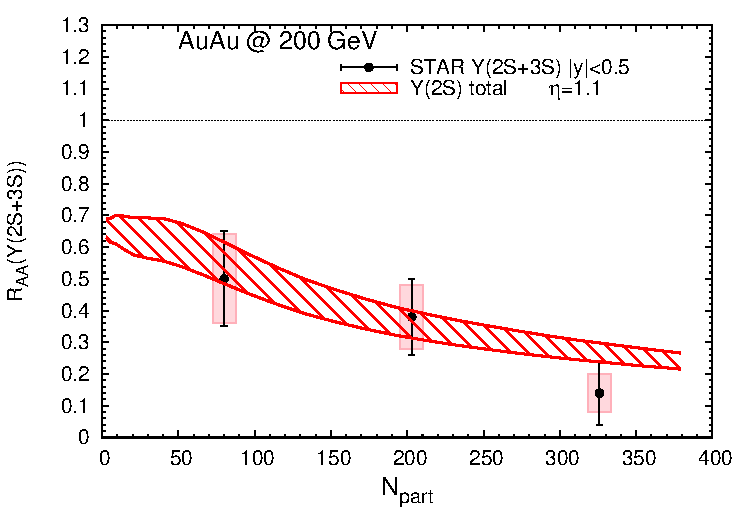
\includegraphics[width=0.48\textwidth]{Figures/fig1_rapp.pdf}
%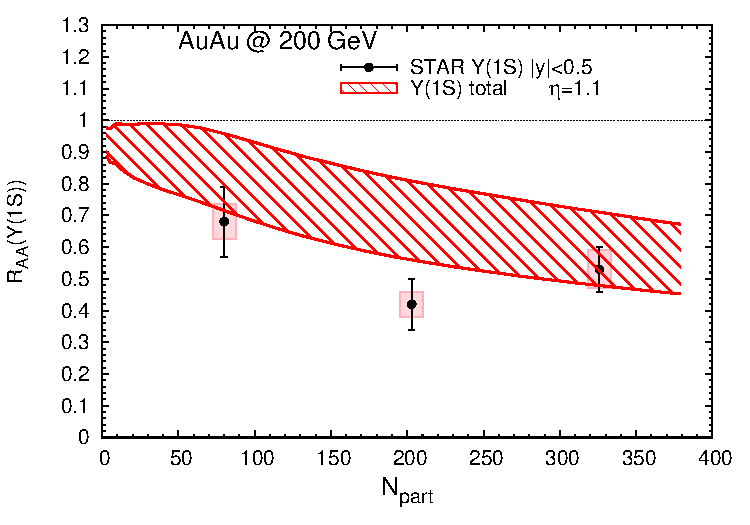
\includegraphics[width=0.48\textwidth]{Figures/fig2_rapp.pdf}
%\caption{Centrality dependence of the $R_{\rm AA}$ for
%$\Upsilon(1S)$ (left) and $\Upsilon(2S)$ (right)
%in 200\,GeV Au-Au collisions at RHIC, compared to
%STAR data~\cite{Ye:2017qmstar}. The uncertainty bands are due to CNM effects represented by nuclear absorption cross sections, $\sigma_Y^{\rm abs}$=0-3\,mb. Figure taken from~\cite{rappqm17}.}
%\label{fig_star}
%\end{figure}

\begin{figure}[t]
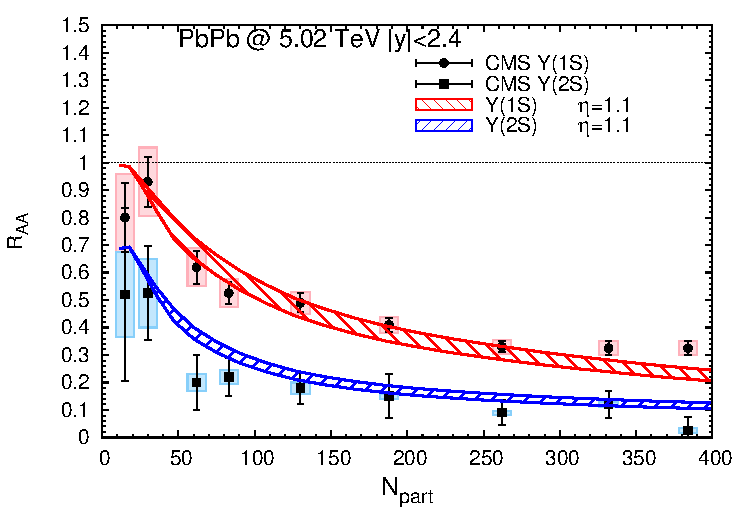
\includegraphics[width=0.49\textwidth]{Figures/fig3_rapp.pdf}
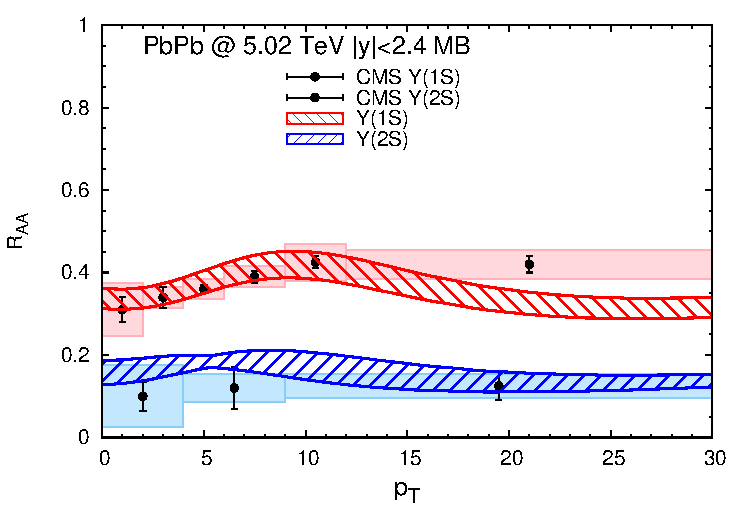
\includegraphics[width=0.49\textwidth]{Figures/fig4_rapp.pdf}
\caption{Centrality (left) and transverse-momentum (right) dependence of the $R_{\rm AA}$ for $\Upsilon(1S)$ and $\Upsilon(2S)$ in 5.02\,TeV Pb-Pb collisions at the LHC, compared to CMS data~\cite{Flores:2017qmcms}. The bands represent a 0-15\,\% shadowing~\cite{Eskola:2009uj} on open-bottom and bottomonia.}
\label{fig_cms}
\end{figure}

Figure \ref{fig_cms} shows the results contrasted with the mid-rapidity data of STAR (at
$\sqrt{s}$=200\,GeV)~\cite{Ye:2017qmstar} and CMS
(at $\sqrt{s}$=5.02\,TeV)~\cite{Flores:2017qmcms}, respectively. 
The authors of this model found a reasonable agreement  with experimental data for the centrality dependence of both $\Upsilon(1S)$ and $\Upsilon(2S)$ at both collision energies. Interestingly they could reproduce the strong suppression of
 the $\Upsilon(2S)$ observed by STAR.  
The calculated $p_T$ spectra at 5.02\,TeV appear to capture the rather flat shapes in the CMS data. 



\subsection{Suppression in anisotropic medium}



In a series of papers~\cite{Strickland:2011aa,Krouppa:2016jcl,Krouppa:2018lkt} people have studied bottomonia suppression using anisotropic hydrodynamics. 
There are two major {\it new} ingredients to this work : (1) the first-principles calculation of the thermal widths of heavy quarkonium states 
and (2) consideration of the momentum anisotropy of the plasma. 

In these works the phase-space distribution of gluons in the local rest frame is assumed to be 

\begin{equation} 
f({\bf x},{\bf p}) = f_{\rm iso}\left(\sqrt{{\bf p}^2+ \xi({\bf p}\cdot{\bf n})^2 }  / 
p_{\rm hard} \right) 
\label{distribution}
\end{equation} 
In the above equation $\xi$ is a measure of the degree of anisotropy of the plasma given as 
%\begin{equation}
$\xi = \frac{1}{2} \langle 
{\bf p}_\perp^2\rangle/\langle p_z^2\rangle -1$
%\end{equation} 
where $p_z$ and 
${\bf p}_\perp $ are the partonic longitudinal and transverse momenta in the local
rest frame, respectively. In equation \ref{distribution}, $p_{\rm hard}$ is the momentum  
scale of the particles and can be identified with the temperature
in an isotropic plasma. 

An approximate form of the real perturbative heavy quark potential as function of $\xi$ can be 
written as~\cite{Dumitru:2007hy} (for $N_c=3$ and $N_f=2$). 
\begin{eqnarray}
Re[V_{\rm pert}] &=& - \alpha \exp(-\mu r)/r \nonumber \\
\left(\frac{\mu}{m_D}\right)^{-4} &=&  
1 + \xi\left(1 + \frac{\sqrt{2}(1+\xi)^2\left(\cos(2\theta) - 1 \right)}{(2+ \xi)^{5/2}} \right) 
\label{eq:muparam}
\end{eqnarray}
where $\alpha = 4\alpha_s/3$, $m_D^2 = (1.4)^2 16 \pi \alpha_s  \, p_{\rm hard}^2/3$ is the isotropic
Debye mass and $\theta$ is the angle with respect to the beamline.  
The factor of $(1.4)^2$ accounts for higher-order corrections to the isotropic Debye 
mass \cite{Kaczmarek:2004gv}.

This perturbative potential, given in equation (\ref{distribution}) is modified to include the non-perturbative (long range) contributions. 
The modified real part of the potential is given as~\cite{Dumitru:2007hy} 


%
\begin{equation} 
\label{eq:repot}
Re[V] = -\frac{\alpha}{r} \left(1+\mu \, r\right) \exp\left( -\mu
\, r  \right) + \frac{2\sigma}{\mu}\left[1-\exp\left( -\mu
\, r  \right)\right] 
 - \sigma \,r\, \exp(-\mu\,r)- \frac{0.8 \, \sigma}{m_Q^2\, r} \, ,
\end{equation}
%
where the last term is a temperature- and spin-independent quark mass correction 
\cite{Bali:1997am} and $\sigma = 0.223$ GeV is the string tension.  Here  $\alpha$ 
is chosen to be  $0.385$ 
to match zero temperature
binding energy data for heavy quark states \cite{Dumitru:2007hy}.
The imaginary part of the potential is taken as the same as the perturbative heavy quark
potential up to linear order in $\xi$ 
%
\begin{equation} 
Im[V_{\rm pert}] = -\alpha p_{\rm hard} \biggl\{ \phi(\hat{r}) - \xi \left[\psi_1(\hat{r},
\theta)+\psi_2(\hat{r}, \theta)\right]\biggr\} ,
\label{eq:impot}
\end{equation}
%
where $\hat{r}=m_D r$ and $\phi$, $\psi_1$, and $\psi_2$ are defined in Ref.~\cite{Krouppa:2016jcl}. 

 The full model potential, given by $V = Re[V] + i Im[V]$, is used to 
solve the Schr\"odinger equation. 
Solution of the Schr\"odinger equation gives the real and imaginary parts of 
the binding energy of the states.  The imaginary part defines the instantaneous width of the state
$Im[E_{\rm bind}(p_{\rm hard},\xi)] \equiv -\Gamma_T(p_{\rm hard},\xi)/2$. 
The resulting width $\Gamma_T(\tau)$ implicitly depends on the initial temperature of the
system.

The following rate equation is used to account for in-medium bottomonia state decay,
%
\begin{equation} \label{eq:rate}
\frac{dn(\tau,{\bf x}_\perp,\varsigma)}{d\tau} = -\Gamma(\tau,{\bf x}_\perp,\varsigma)n(\tau,{\bf x}_\perp,\varsigma) ,
\end{equation}
%
where   $\tau = \sqrt{t^{2} - z^{2}}$ is the longitudinal proper time,  ${\bf x}_{\perp}$ is the the transverse coordinate and 
 $\varsigma = {\rm arctanh}(z/t)$ is the the spatial rapidity. The rate of decay is computed by~\cite{Strickland:2011aa}
%
\begin{eqnarray}
\Gamma(\tau, {\bf x}_{\perp}, \varsigma) = 
%\begin{cases} 
&2Im[E_{\text{bind}}(\tau, {\bf x}_{\perp}, \varsigma)] & \ \ Re[E_{\text{bind}}(\tau, {\bf x}_{\perp}, \varsigma)] > 0 \\ 
&=\gamma_{\text{dis}} & \ \ Re[E_{\text{bind}}(\tau, {\bf x}_{\perp}, \varsigma)] \leq 0. 
%\end{cases}
\end{eqnarray}
%
In order to look at the suppression one has to calculate $R_{AA}$. The algorithm to obtain $R_{AA}$ is the following. 
First one obtains 
\begin{equation}
 \bar{\gamma}({\bf x}_\perp,p_T,
\varsigma,b) \equiv \Theta(\tau_f-\tau_{\rm form}(p_T)) \int_{{\rm max}(\tau_{\rm form}(p_T),\tau_0)}^{\tau_f} 
d\tau\,\Gamma_T(\tau,{\bf x}_\perp,\varsigma,b) 
\end{equation}
where $\varsigma$ is the spatial
rapidity.  From this one obtains  
\begin{equation}
R_{AA}({\bf x}_\perp,p_T,\varsigma,b) =% 
\exp\!\left(-\bar{\gamma}({\bf x}_\perp,p_T,\varsigma,b) \right)
\end{equation}
  Finally, one averages
over ${\bf x}_\perp$ to obtain 
\begin{equation}
\langle R_{AA}(p_T,\varsigma,b) \rangle \equiv 
[\int_{{\bf x}_\perp} \! d{\bf x}_\perp \, T_{AA}({\bf x}_\perp)\,%
R_{AA}({\bf x}_\perp,p_T,\varsigma,b)]/[\int_{{\bf x}_\perp} \! d{\bf x}_\perp \,% 
T_{AA}({\bf x}_\perp)]
\end{equation} 

\begin{figure}[t]
\begin{center}
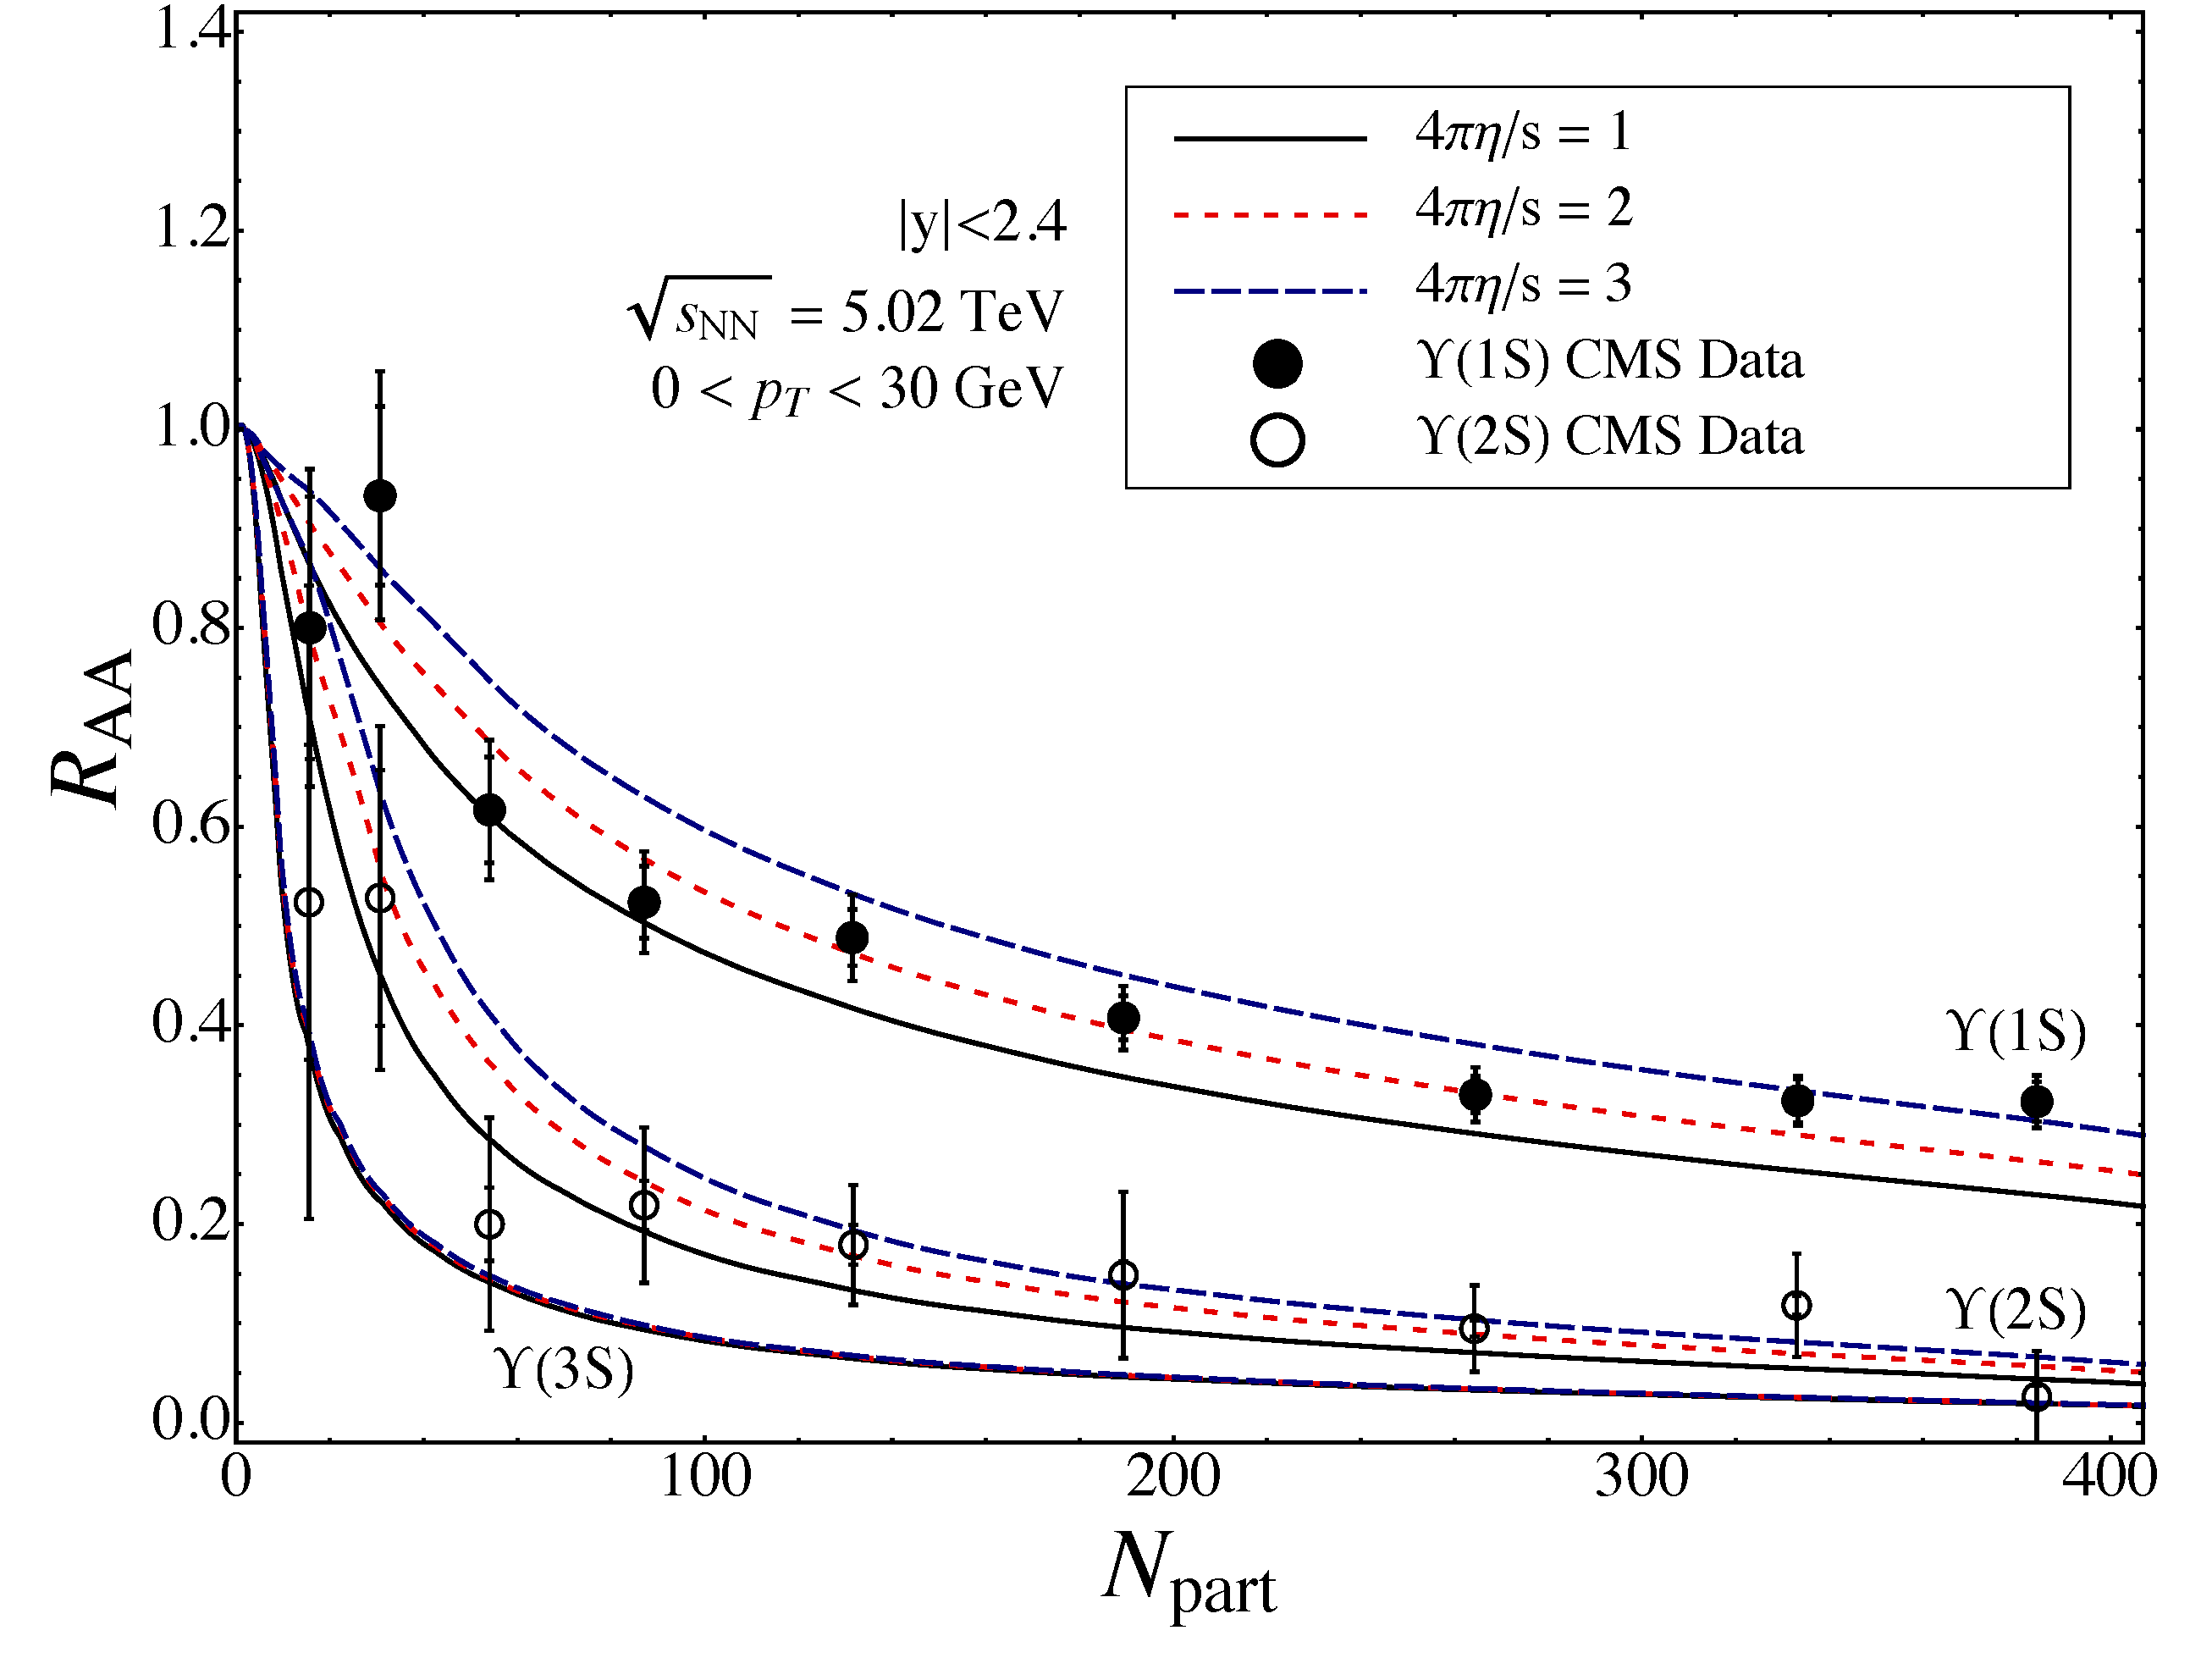
\includegraphics[width=0.5\textwidth]{Figures/CMS-SB.pdf}
\end{center}
\vspace{-7mm}
\caption{Calculation for the inclusive $\Upsilon(nS)$ curves as a function of $N_{\text{part}}$. A comparison is made for the CMS experiment at the LHC.}

\label{fig:raasep}
\end{figure}


In Fig.~\ref{fig:raasep} the $R_{AA}$ for $\Upsilon(1s)$ and $\chi_{b1}$ has been plotted 
as a function of $N_{\rm part}$.  The authors have depicted that there is substantial 
suppression  of $\Upsilon(1s)$ which they have accounted to the in-medium decay.  
A  similar suppression pattern is observed for  $\chi_{b1}$.  This may be attributed to the 
finite formation time of the $\chi_{b1}$. 


%In a series of papers [ .... References .....]
%people have studied bottomonia suppression using anisotropic hydrodynamics. 
%There are two major {\it new} ingredients to this work : (1) the first-principles calculation of the thermal widths of heavy quarkonium states 
%and (2) consideration of the momentum anisotropy of the plasma. 

%In these works the phase-space distribution of gluons in the local rest frame is assumed to be 

%\begin{equation} 
%f({\bf x},{\bf p}) = f_{\rm iso}\left(\sqrt{{\bf p}^2+ \xi({\bf p}\cdot{\bf n})^2 }  / 
%p_{\rm hard} \right) 
%\label{distribution}
%\end{equation} 
%In the above equation $\xi$ is a measure of the degree of anisotropy of the plasma.
%\begin{equation}
%\xi = \frac{1}{2} \langle 
%{\bf p}_\perp^2\rangle/\langle p_z^2\rangle -1
%\end{equation} 
%where $p_z$ and 
%${\bf p}_\perp $ are the partonic longitudinal and transverse momenta in the local
%rest frame, respectively. In equation \ref{distribution}, $p_{\rm hard}$ is the momentum  
%scale of the particles and can be identified with the temperature
%5in an isotropic plasma. 

%An approximate form of the real perturbative heavy quark potential as function of $\xi$ can be 
%written as~\cite{Dumitru:2007hy} (for $N_c=3$ and $N_f=2$). 
%\begin{eqnarray}
%Re[V_{\rm pert}] &=& - \alpha \exp(-\mu r)/r \nonumber \\
%\left(\frac{\mu}{m_D}\right)^{-4} &=&  
%1 + \xi\left(1 + \frac{\sqrt{2}(1+\xi)^2\left(\cos(2\theta) - 1 \right)}{(2+ \xi)^{5/2}} \right) 
%\label{eq:muparam}
%\end{eqnarray}
%where $\alpha = 4\alpha_s/3$, $m_D^2 = (1.4)^2 16 \pi \alpha_s  \, p_{\rm hard}^2/3$ is the isotropic
%Debye mass and $\theta$ is the angle with respect to the beamline.  
%The factor of $(1.4)^2$ accounts for higher-order corrections to the isotropic Debye 
%mass \cite{Kaczmarek:2004gv}.

%This perturbative potential, given in equation (\ref{distribution}) is modified to include the non-perturbative (long range) contributions. 
%The modified real part of the potential is given as~\cite{Dumitru:2007hy} 


%
%\begin{eqnarray} 
%\label{eq:repot}
%Re[V] &=& -\frac{\alpha}{r} \left(1+\mu \, r\right) \exp\left( -\mu
%\, r  \right) + \frac{2\sigma}{\mu}\left[1-\exp\left( -\mu
%\, r  \right)\right] \nonumber \\
%&& \hspace{2cm} - \sigma \,r\, \exp(-\mu\,r)- \frac{0.8 \, \sigma}{m_Q^2\, r} \, ,
%\end{eqnarray}
%
%where the last term is a temperature- and spin-independent quark mass correction 
%\cite{Bali:1997am} and $\sigma = 0.223$ GeV is the string tension.  Here  $\alpha$ 
%is chosen to be  $0.385$ 
%to match zero temperature
%binding energy data for heavy quark states \cite{Dumitru:2007hy}.
%The imaginary part of the potential is taken as the same as the perturbative heavy quark
%potential up to linear order in $\xi$ 
%
%\begin{equation} 
%Im[V_{\rm pert}] = -\alpha p_{\rm hard} \biggl\{ \phi(\hat{r}) - \xi \left[\psi_1(\hat{r},
%\theta)+\psi_2(\hat{r}, \theta)\right]\biggr\} ,
%\label{eq:impot}
%\end{equation}
%%
%where $\hat{r}=m_D r$ and $\phi$, $\psi_1$, and $\psi_2$ are defined as

%%The full model potential is given by $V = Re[V] + i Im[V]$ and can be used in the Schr\"odinger equation. 

%\begin{equation}
%\phi(\hat{r}) = 2\int_{0}^{\infty} dz \frac{z}{(z^2+1)^2}\left[1-\frac{\sin\left(z\hat{r}\right)}{\hat{r}}\right],
%\end{equation}

%\begin{equation}
% \psi_1(\hat{r}, \theta) = \int_0^{\infty} dz
% \frac{z}{(z^2+1)^2}\left(1-\frac{3}{2}
% \left[\sin^2\theta\frac{\sin(z\, \hat{r})}{z\, \hat{r}}
% +(1-3\cos^2\theta)G(\hat{r}, z)\right]\right),
% \end{equation}

 %\begin{equation}
 %\psi_2(\hat{r}, \theta) = - \int_0^{\infty} dz
%\frac{\frac{4}{3}z}{(z^2+1)^3}\left(1-3 \left[
%  \left(\frac{2}{3}-\cos^2\theta \right) \frac
% {\sin(z\, \hat{r})}{z\, \hat{r}}+(1-3\cos^2\theta)
% G(\hat{r},z)\right]\right).
%\label{eq:psis}
%\end{equation}
%where $G(\hat{r},z)$ is the Meijer G-function. The full model potential, given by $V = Re[V] + i Im[V]$, is used to 
%solve the Schr\"odinger equation. 


%Solution of the Schr\"odinger equation gives the real and imaginary parts of 
%the binding energy of the states.  The imaginary part defines the instantaneous width of the state
%$Im[E_{\rm bind}(p_{\rm hard},\xi)] \equiv -\Gamma_T(p_{\rm hard},\xi)/2$. 
%The resulting width $\Gamma_T(\tau)$ implicitly depends on the initial temperature of the
%system.

%The following rate equation is used to account for in-medium bottomonia state decay,
%%
%\begin{equation} \label{eq:rate}
%\frac{dn(\tau,{\bf x}_\perp,\varsigma)}{d\tau} = -\Gamma(\tau,{\bf x}_\perp,\varsigma)n(\tau,{\bf x}_\perp,\varsigma) ,
%\end{equation}
%%
%where   $\tau = \sqrt{t^{2} - z^{2}}$ is the longitudinal proper time,  ${\bf x}_{\perp}$ is the the transverse coordinate and 
% $\varsigma = {\rm arctanh}(z/t)$ is the the spatial rapidity. The rate of decay is computed by~\cite{Strickland:2011aa}
%%
%\begin{eqnarray}
%\Gamma(\tau, {\bf x}_{\perp}, \varsigma) = 
%%\begin{cases} 
%&2Im[E_{\text{bind}}(\tau, {\bf x}_{\perp}, \varsigma)] & \ \ Re[E_{\text{bind}}(\tau, {\bf x}_{\perp}, \varsigma)] > 0 \\ 
%&=\gamma_{\text{dis}} & \ \ Re[E_{\text{bind}}(\tau, {\bf x}_{\perp}, \varsigma)] \leq 0. 
%%\end{cases}
%\end{eqnarray}
%%
%In order to look at the suppression one has to calculate $R_{AA}$. The algorithm to obtain $R_{AA}$ is the following. 
%First one obtains 
%\begin{equation}
% \bar{\gamma}({\bf x}_\perp,p_T,
%\varsigma,b) \equiv \Theta(\tau_f-\tau_{\rm form}(p_T)) \int_{{\rm max}(\tau_{\rm form}(p_T),\tau_0)}^{\tau_f} 
%d\tau\,\Gamma_T(\tau,{\bf x}_\perp,\varsigma,b) 
%\end{equation}
%where $\varsigma$ is the spatial
%rapidity.  From this one obtains  
%\begin{equation}
%R_{AA}({\bf x}_\perp,p_T,\varsigma,b) =% 
%\exp\!\left(-\bar{\gamma}({\bf x}_\perp,p_T,\varsigma,b) \right)
%\end{equation}
%  Finally, one averages
%over ${\bf x}_\perp$ to obtain 
%\begin{equation}
%\langle R_{AA}(p_T,\varsigma,b) \rangle \equiv 
%[\int_{{\bf x}_\perp} \! d{\bf x}_\perp \, T_{AA}({\bf x}_\perp)\,%
%R_{AA}({\bf x}_\perp,p_T,\varsigma,b)]/[\int_{{\bf x}_\perp} \! d{\bf x}_\perp \,% 
%T_{AA}({\bf x}_\perp)]
%\end{equation} 

%\begin{figure}[t]
%\begin{center}
%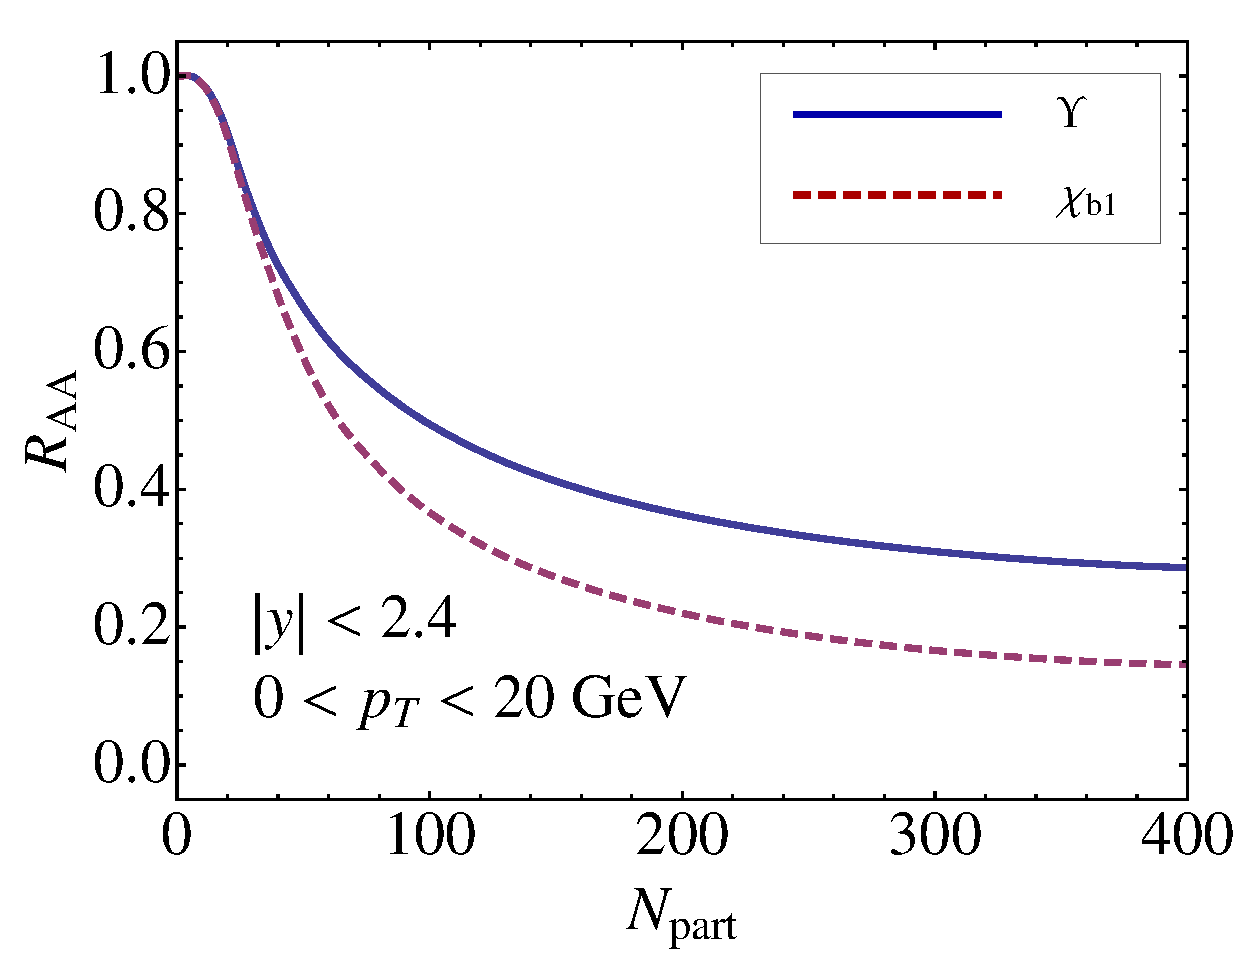
\includegraphics[width=0.6\textwidth]{Figures/fig1_strickland.pdf}
%\end{center}
%\vspace{-7mm}
%\caption{Rapidity- and $p_T$-averaged $R_{AA}$ for $\Upsilon(1s)$ and $\chi_{b1}$ as a function of $N_{\rm part}$ using
%$4 \pi \eta/{\cal S}=1$.}
%\label{fig:raasep}
%\end{figure}


%In Fig.~\ref{fig:raasep} the $R_{AA}$ for $\Upsilon(1s)$ and $\chi_{b1}$ has been plotted 
%as a function of $N_{\rm part}$.  The authors have depicted that there is substantial 
%suppression  of $\Upsilon(1s)$ which they have accounted to the in-medium decay.  
%A  similar suppression pattern is observed for  $\chi_{b1}$.  This may be attributed to the 
%finite formation time of the $\chi_{b1}$. 

%\subsubsection{Non-equilibrium effects on quarkonium suppression}
%\subsubsection{Collisional dissociation of quarkonia from final-state interactions}




%%%%%%%%%%%%%%%%%%%%%%%%%%%%%%%%%%%%%%%%%%%%%%%%%%%%%%%%%%%%%%%%%%%%%%%%%%
